\part{Analyse des cas d'utilisation}
\setcounter{section}{0}

\section{CU1 - Génération de contacts}

\begin{figure}[H]
\centering
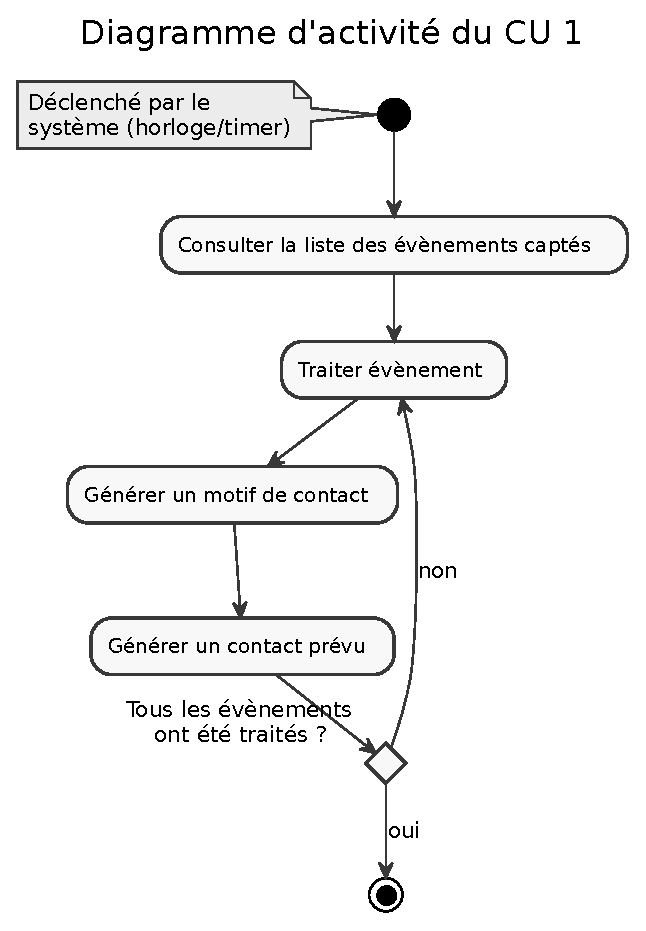
\includegraphics[width=10cm]{figures/eps/DA_CU1.eps}
\caption{DA du CU1}
\end{figure}

\begin{figure}[H]
\noindent\makebox[\textwidth]{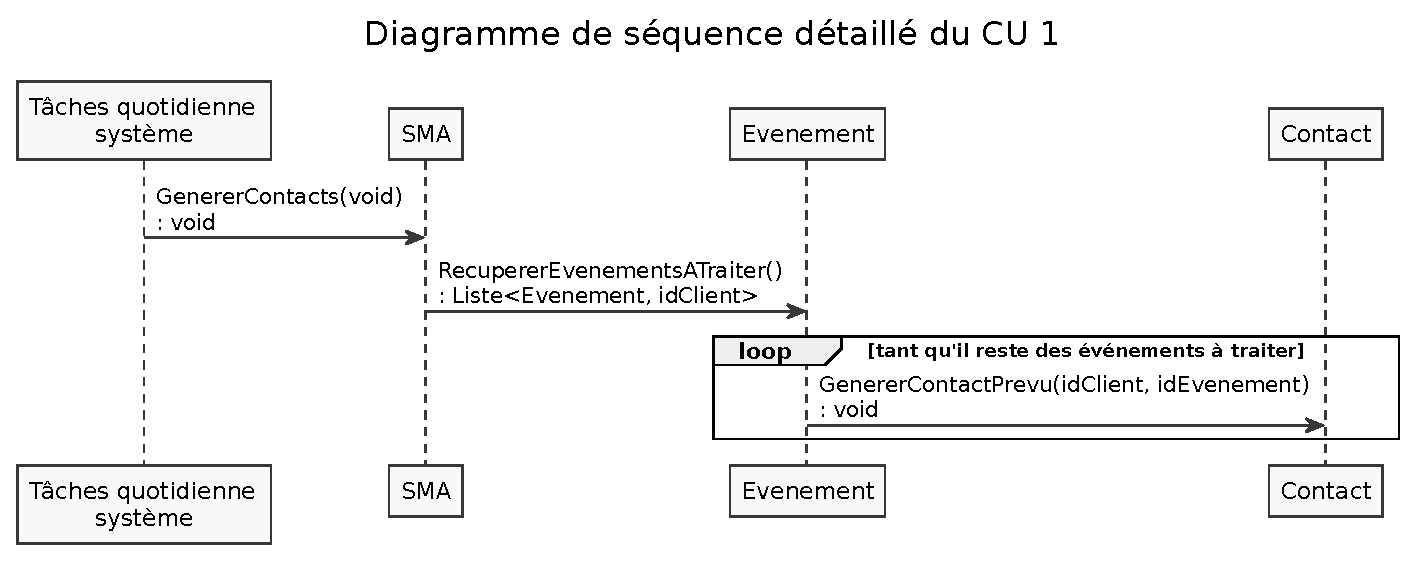
\includegraphics[width=19cm]{figures/eps/DSD_CU1.eps}}
\caption{DSD du CU1}
\end{figure}

\clearpage
\section{CU2 - Répartition des contacts commerciaux}

\begin{figure}[H]
\centering
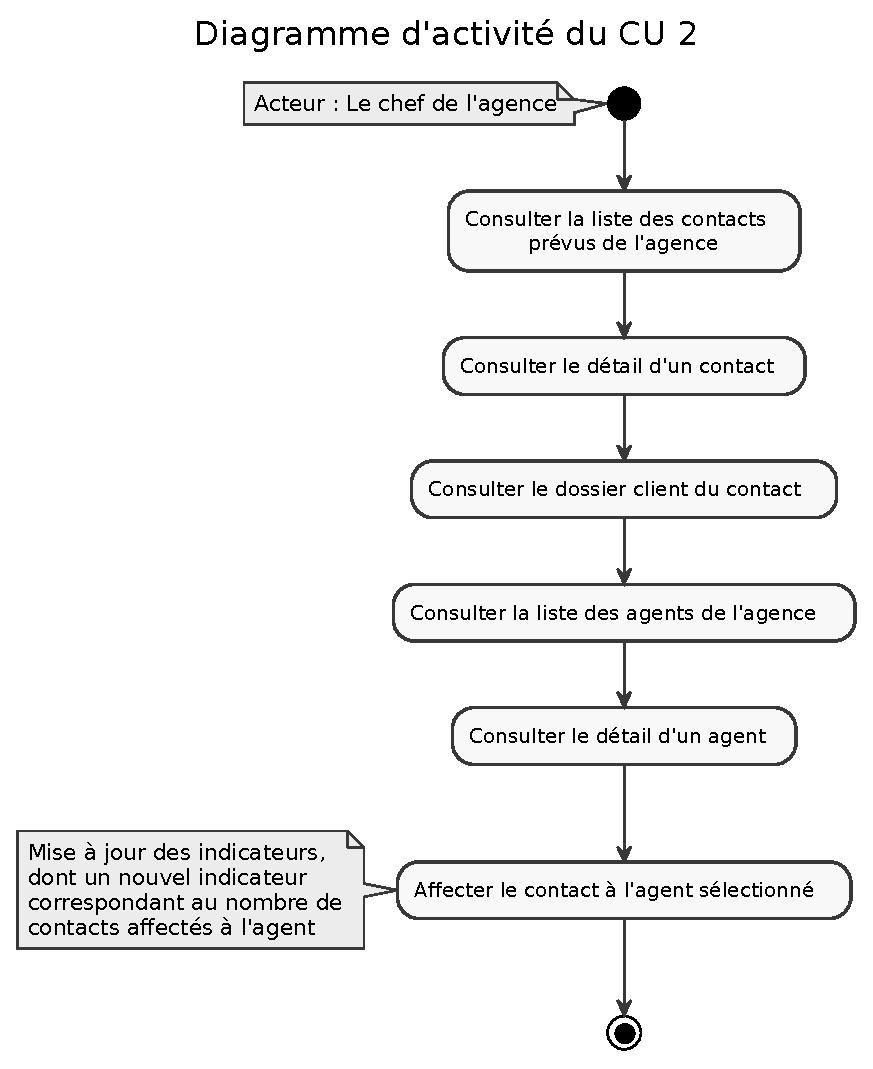
\includegraphics[width=\textwidth]{figures/eps/DA_CU2.eps}
\caption{DA du CU2}
\end{figure}


\begin{figure}[H]
\noindent\makebox[\textwidth]{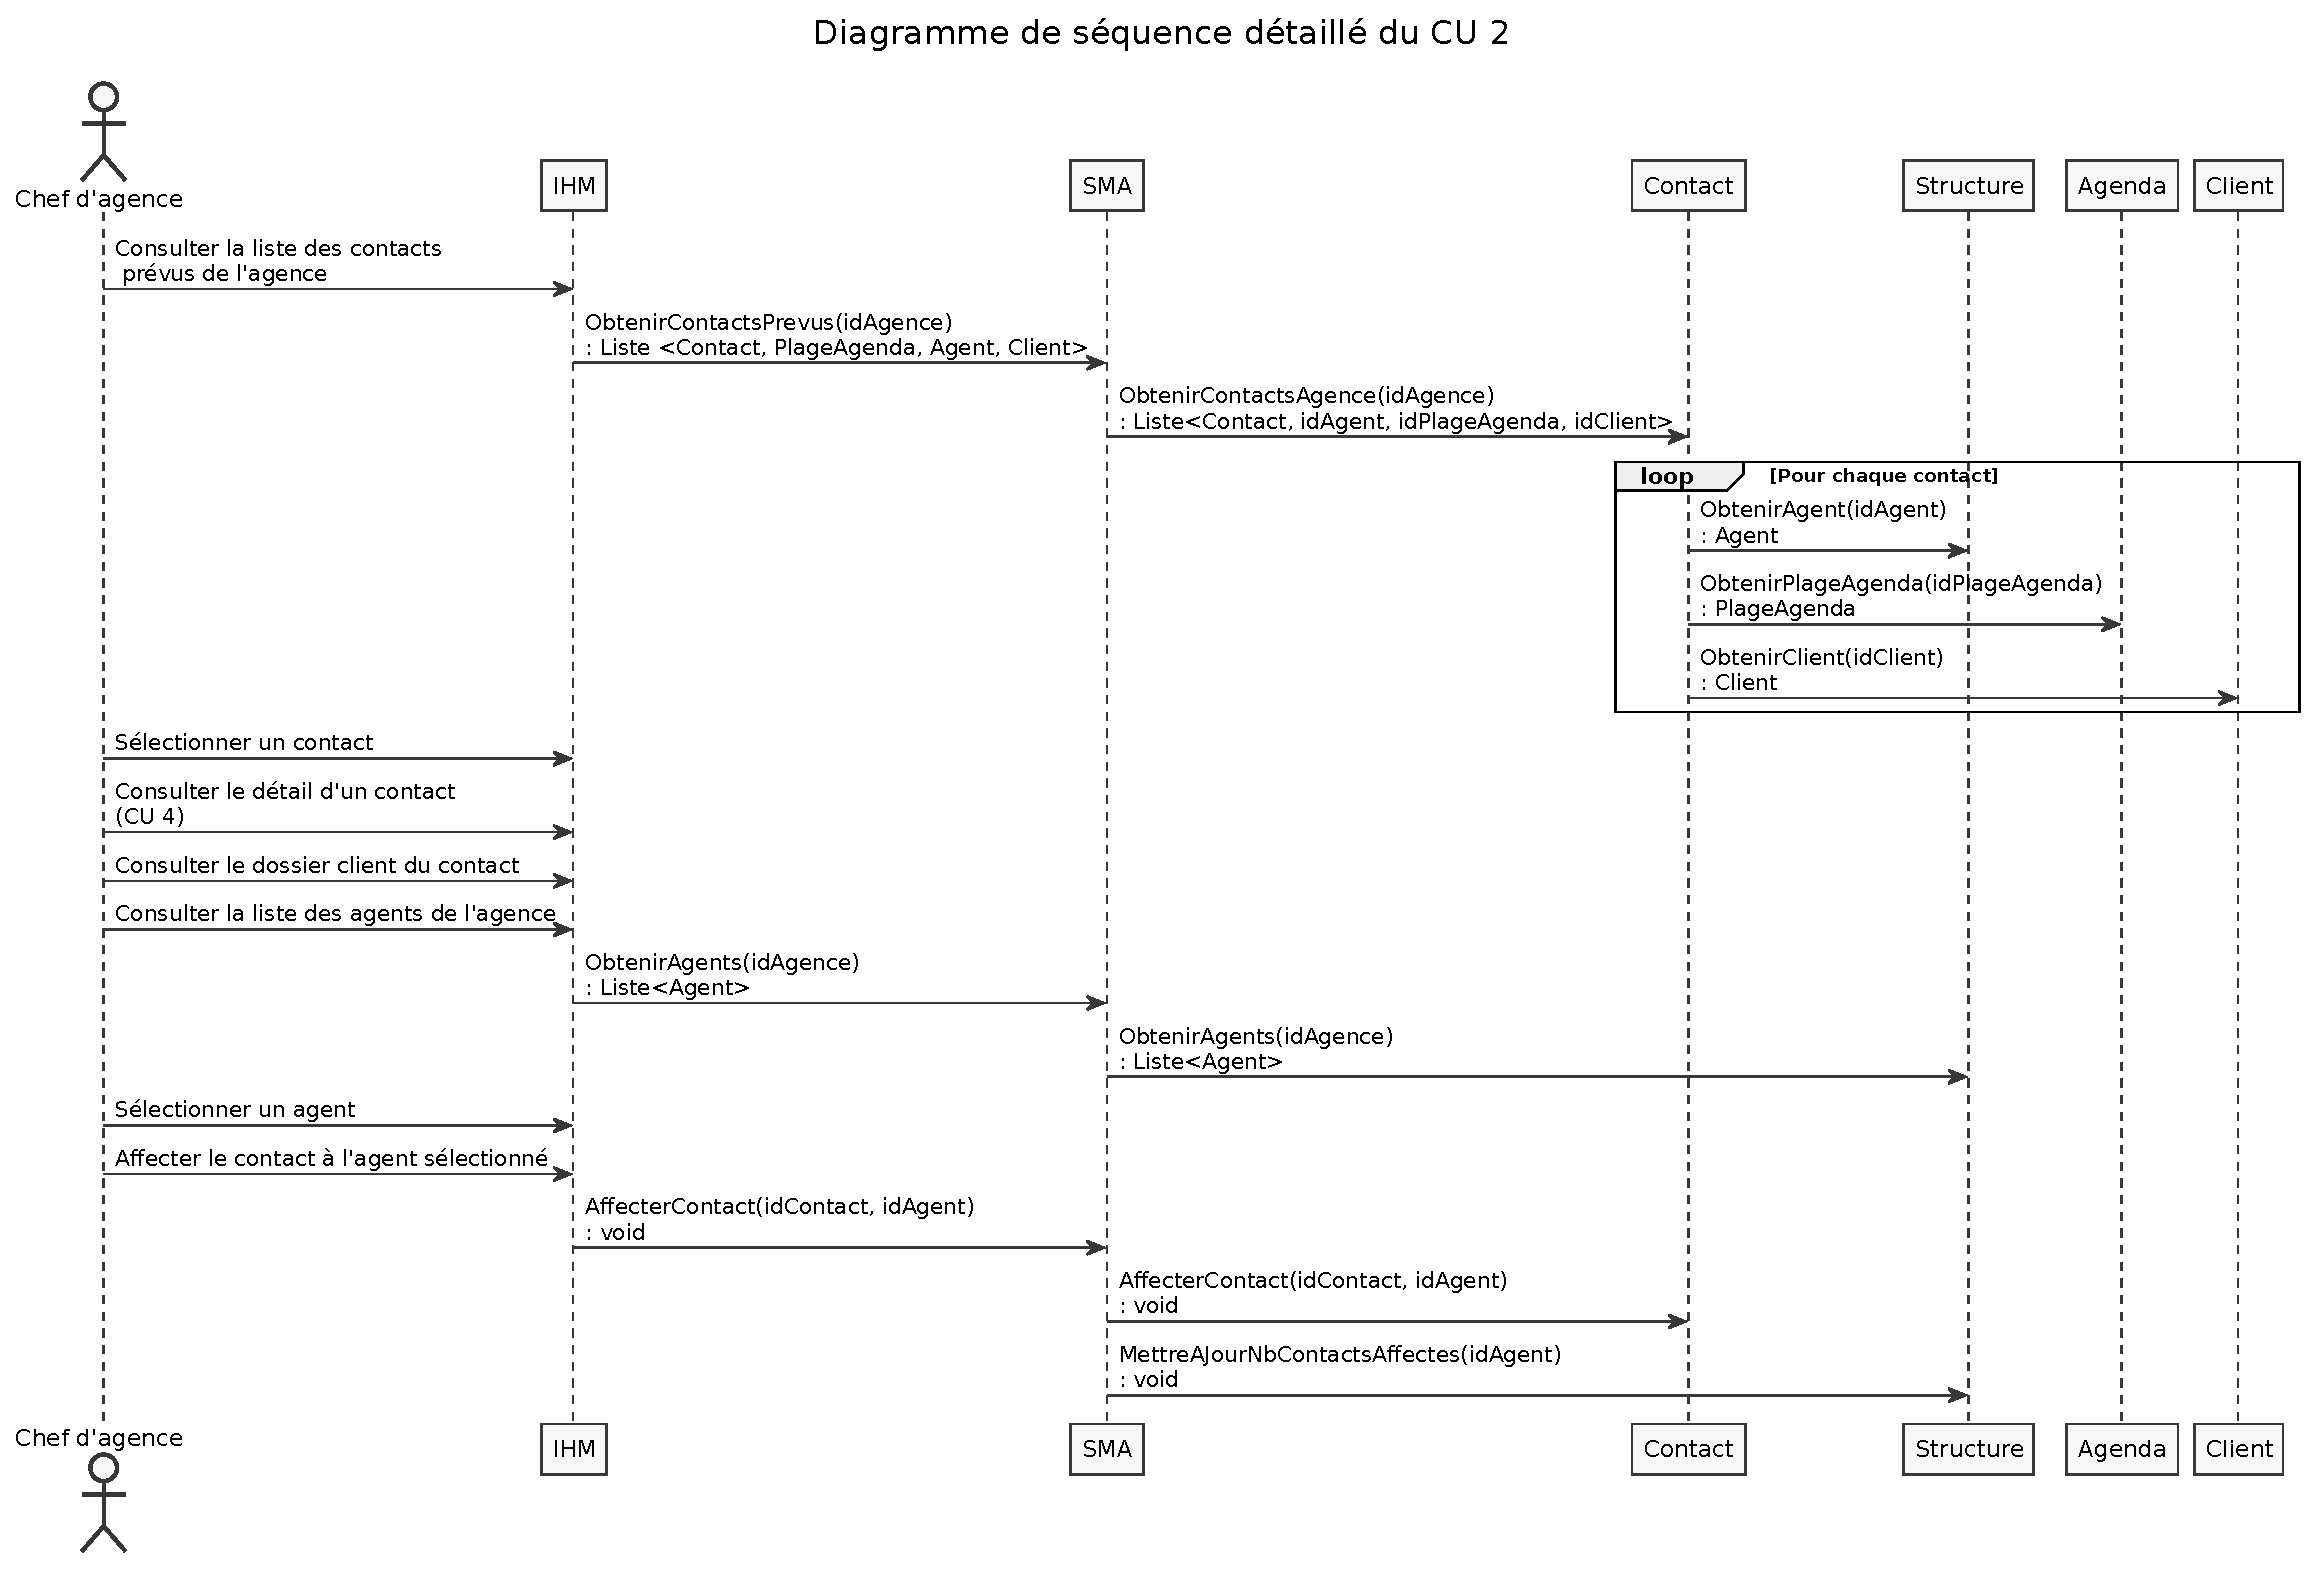
\includegraphics[width=23cm, angle=90]{figures/eps/DSD_CU2.eps}}
\caption{DSD du CU2}
\end{figure}


\clearpage
\section{CU3 - Suivi de l’action commercial}

\begin{figure}[H]
\centering
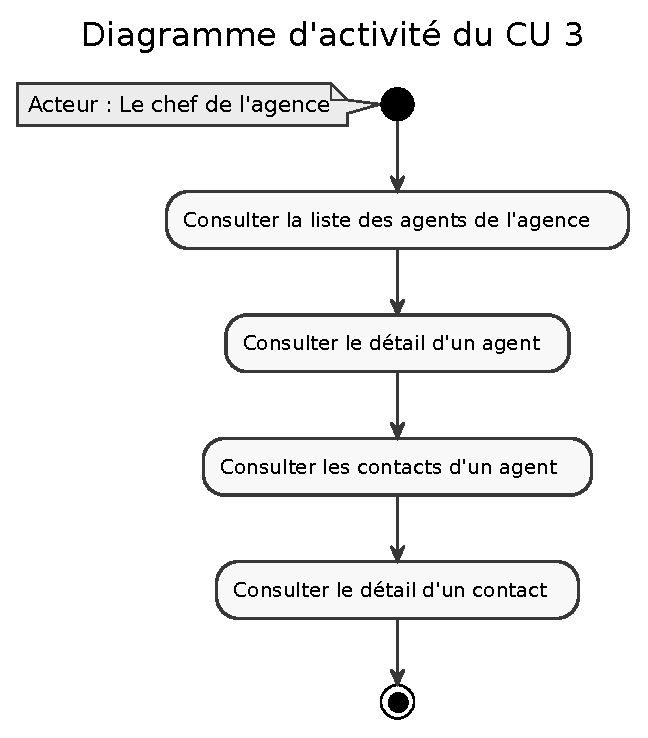
\includegraphics[width=10cm]{figures/eps/DA_CU3.eps}
\caption{DA du CU3}
\end{figure}

\begin{figure}[H]
\centering
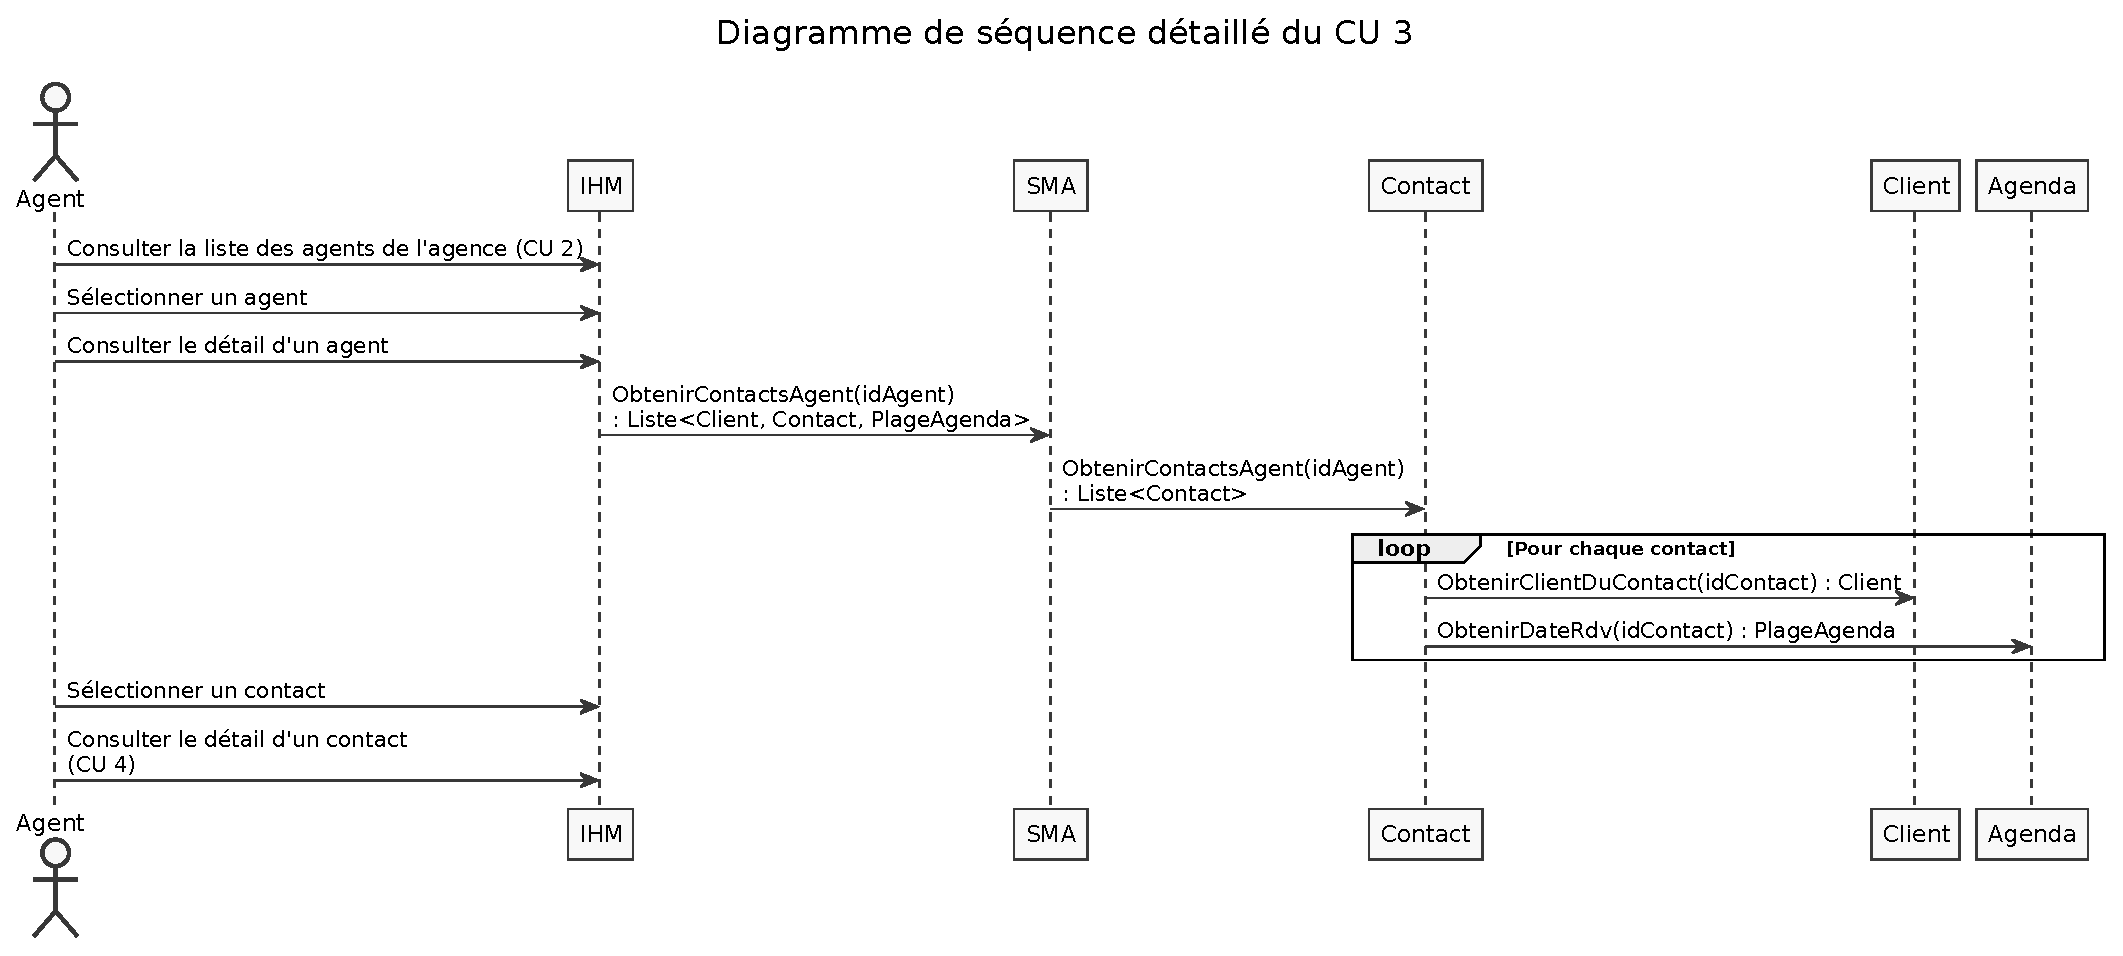
\includegraphics[width=10cm]{figures/eps/DSD_CU3.eps}
\caption{DSD du CU3}
\end{figure}

\clearpage
\section{CU4 – Gestion de la liste des contacts clients}

\begin{figure}[H]
\centering
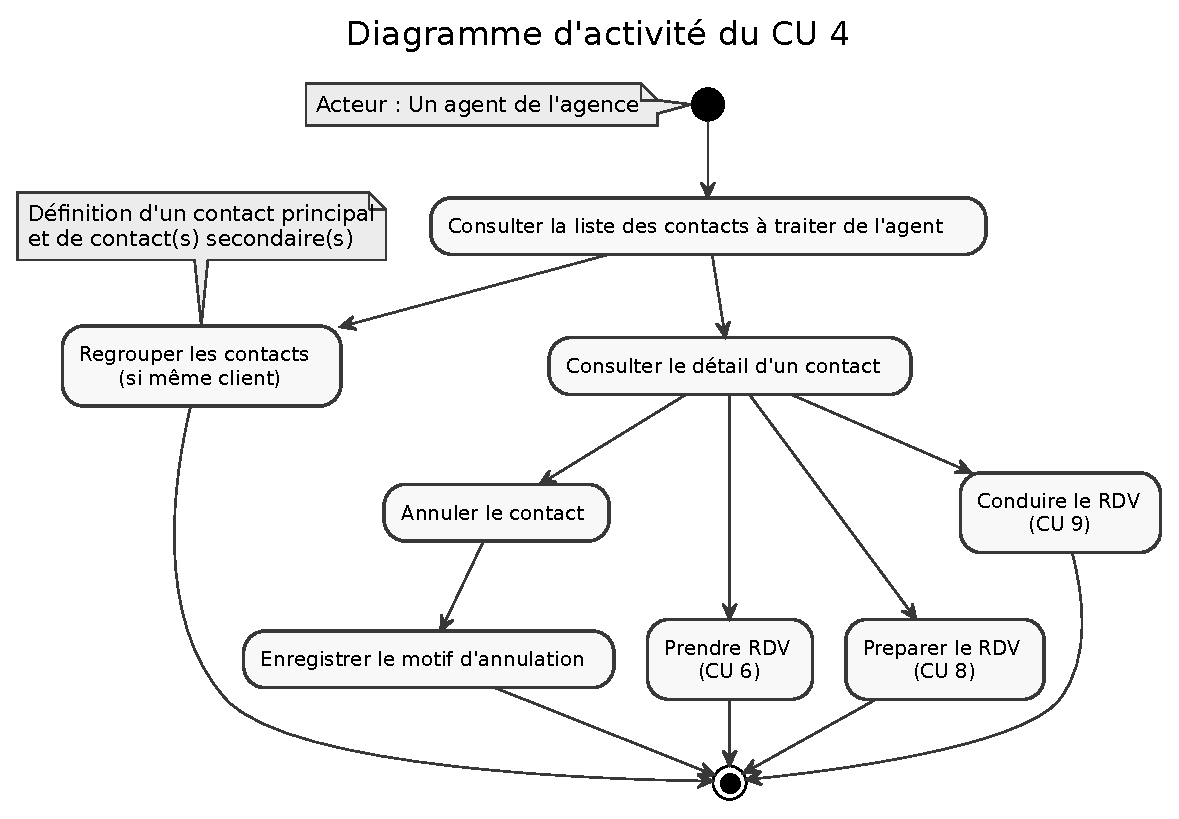
\includegraphics[width=\textwidth]{figures/eps/DA_CU4.eps}
\caption{DA du CU4}
\end{figure}

\begin{figure}[H]
\noindent\makebox[\textwidth]{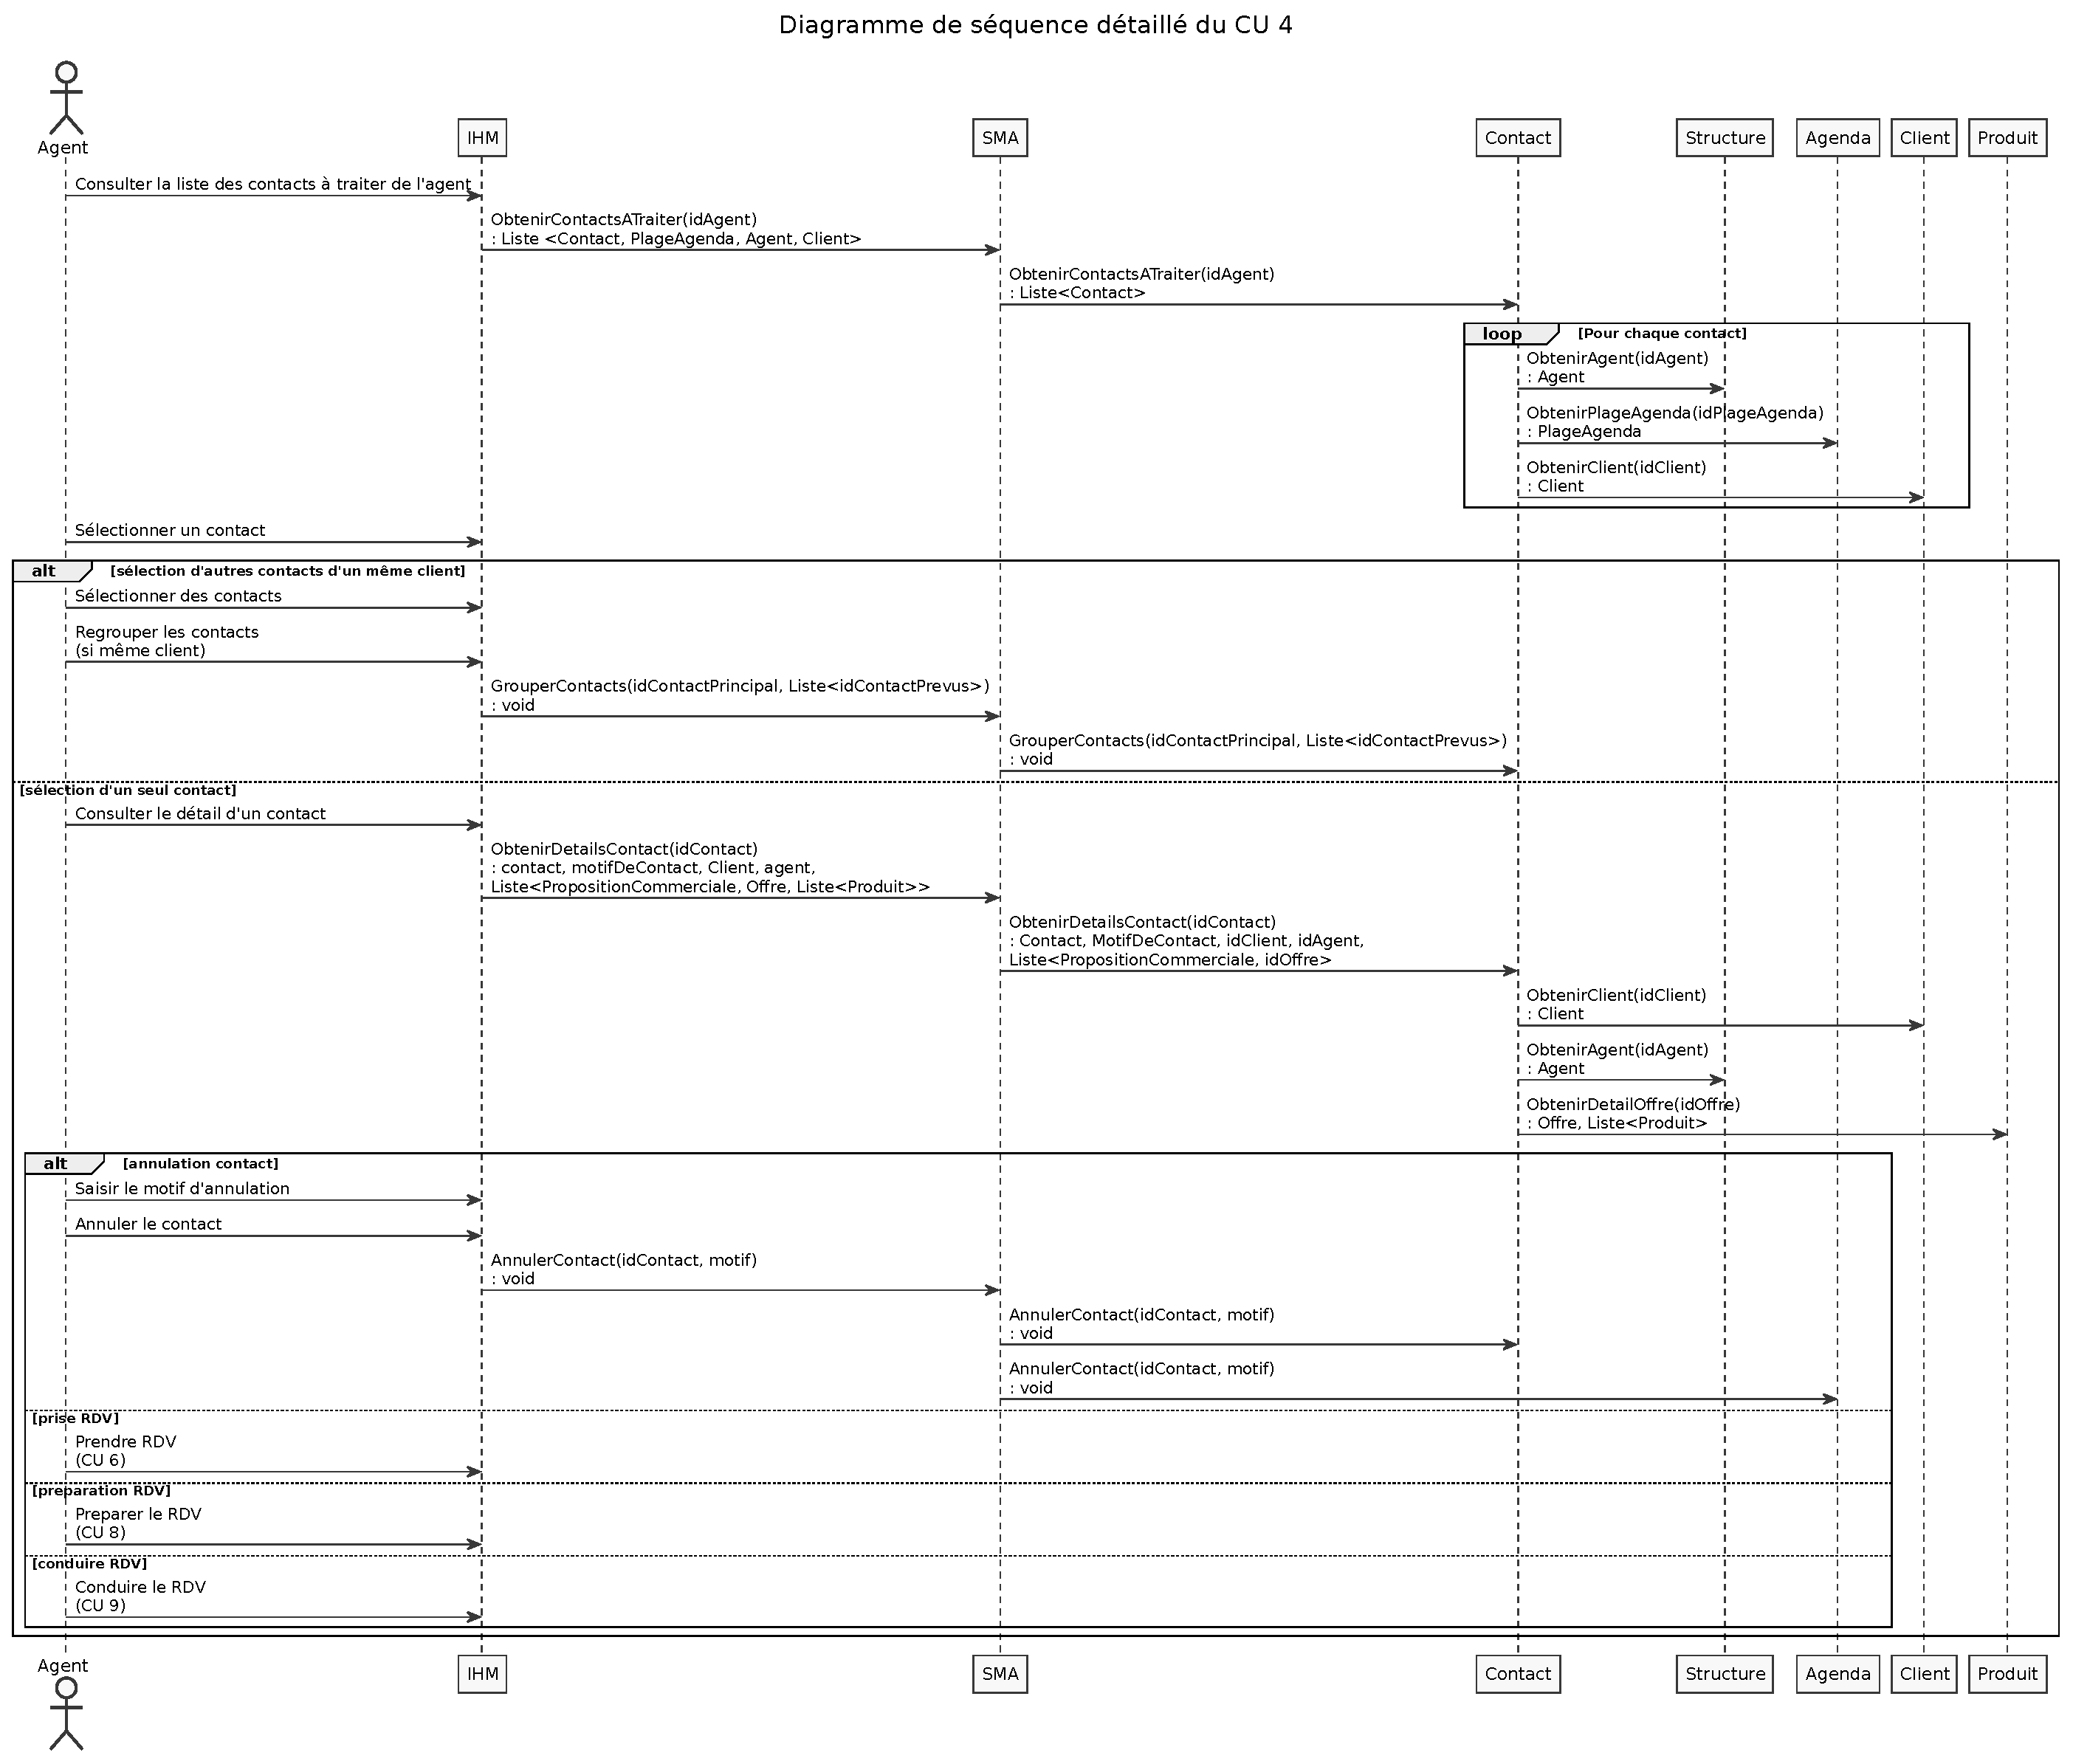
\includegraphics[width=21cm, angle=90]{figures/eps/DSD_CU4.eps}}
\caption{DSD du CU4}
\end{figure}



\clearpage
\section{CU5 - Planification de l’activité de l’agence du mois suivant}

\begin{figure}[H]
\centering
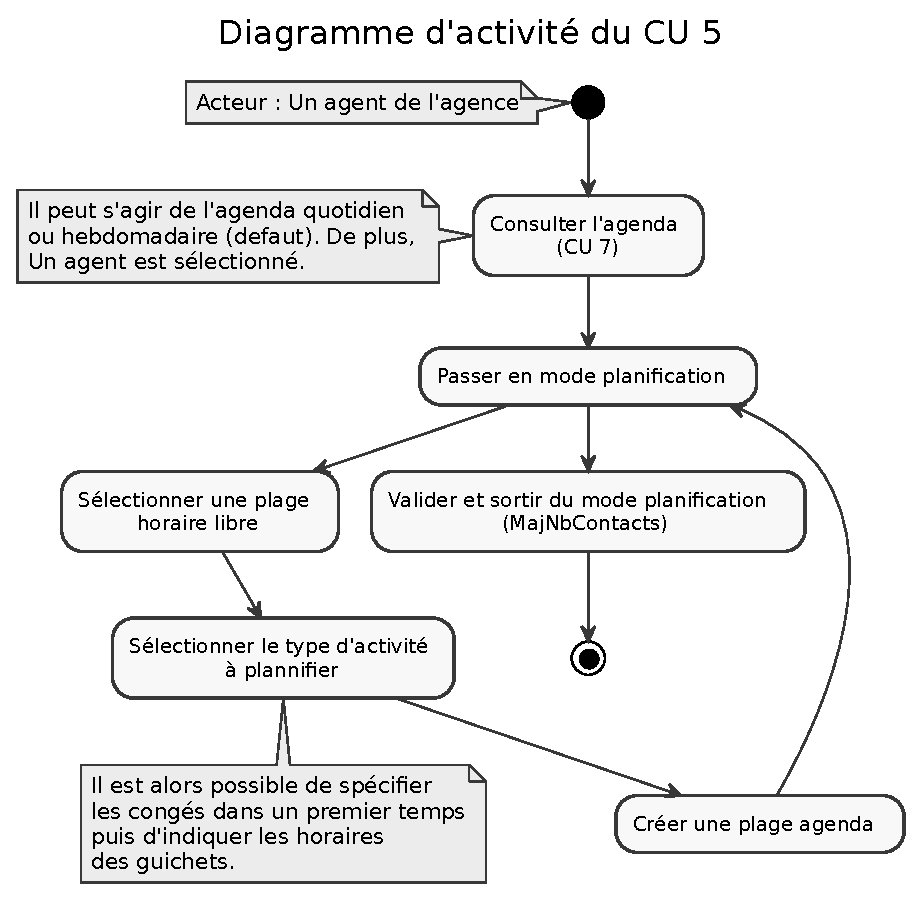
\includegraphics[width=\textwidth]{figures/eps/DA_CU5.eps}
\caption{DA du CU5}
\end{figure}

\begin{figure}[H]
\centering
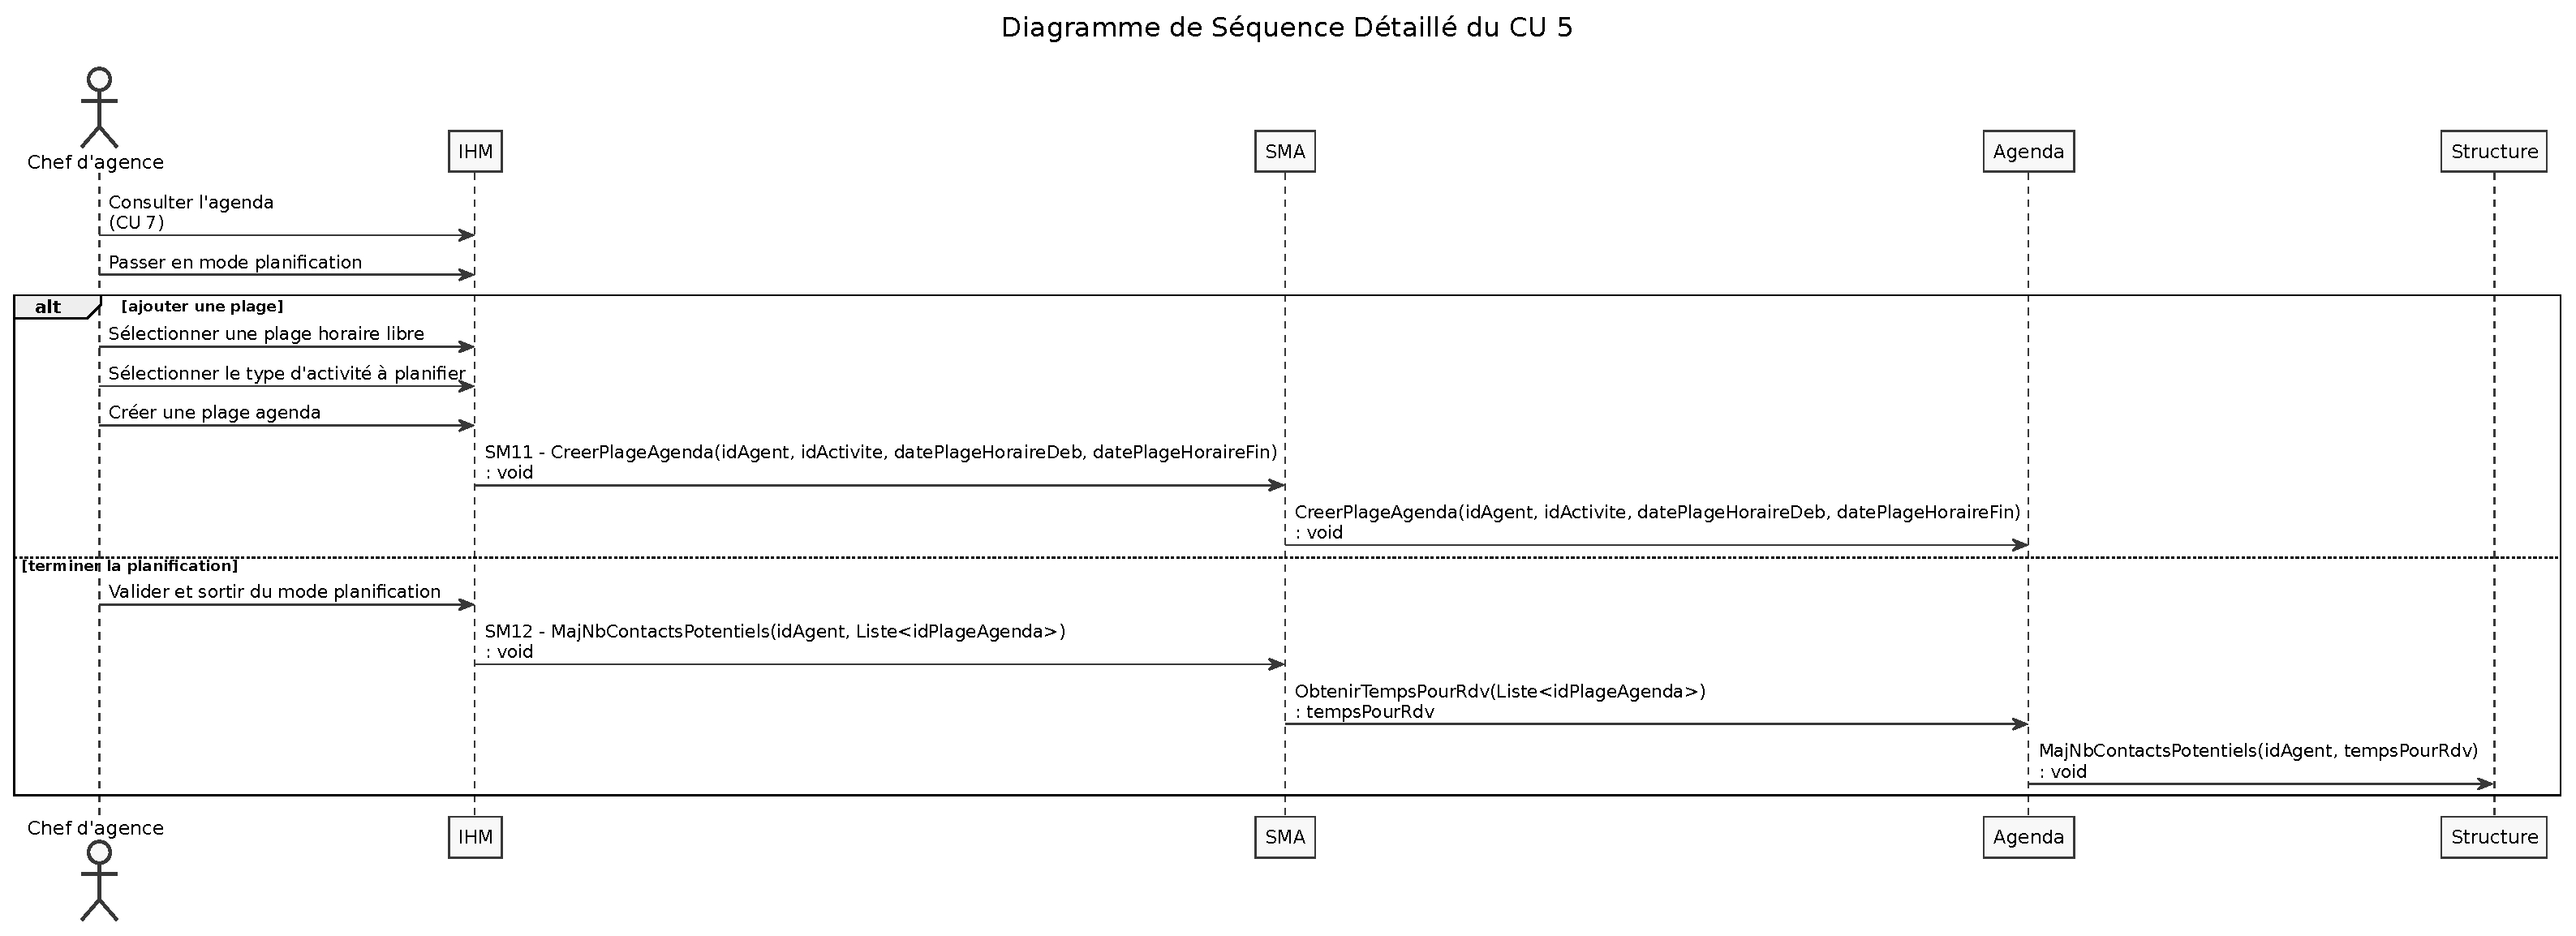
\includegraphics[width=26cm, angle=90]{figures/eps/DSD_CU5.eps}
\caption{DSD du CU5}
\end{figure}

\clearpage
\section{CU6 - Planification des contacts commerciaux}

\subsection{Partie Agent}
\begin{figure}[H]
\centering
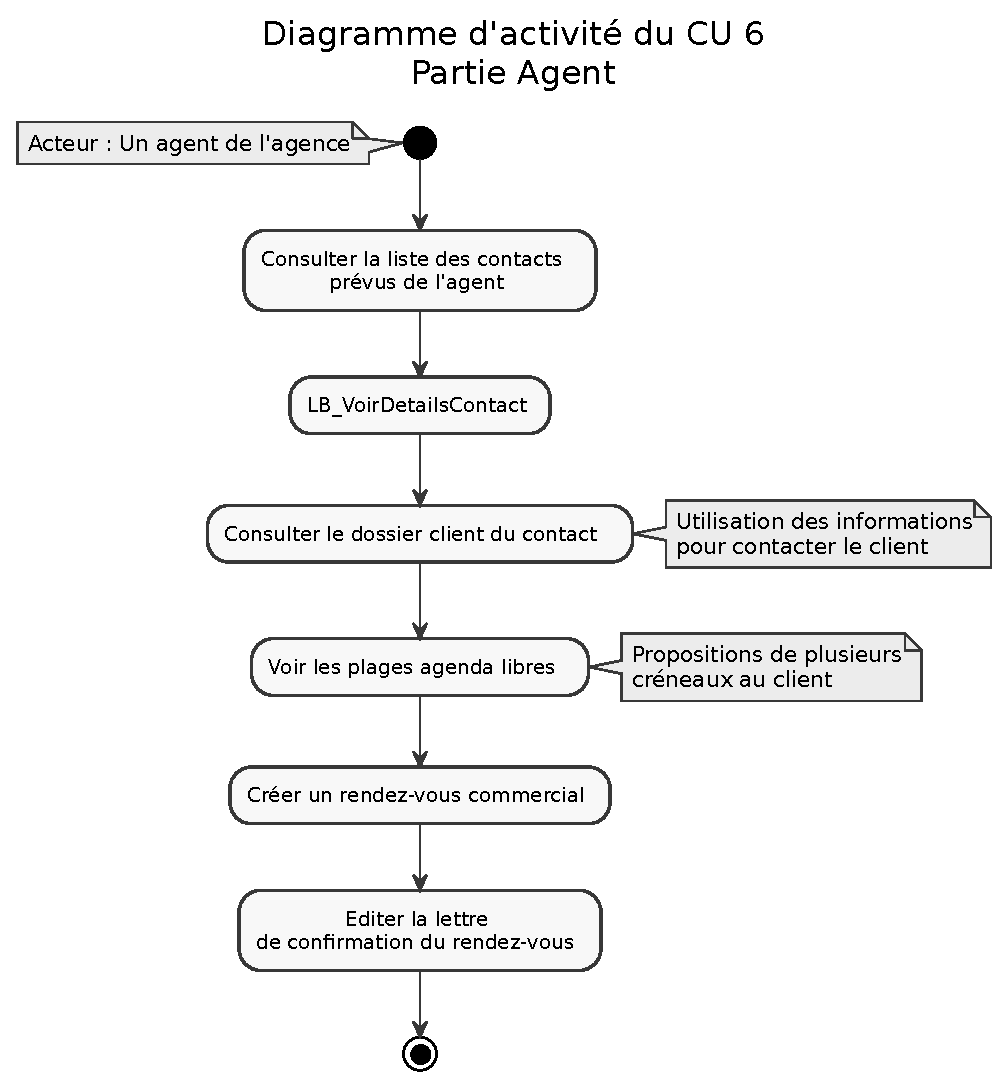
\includegraphics[width=\textwidth]{figures/eps/DA_CU6_partieAgent.eps}
\caption{DA du CU6}
\end{figure}

\begin{figure}[H]
\noindent\makebox[\textwidth]{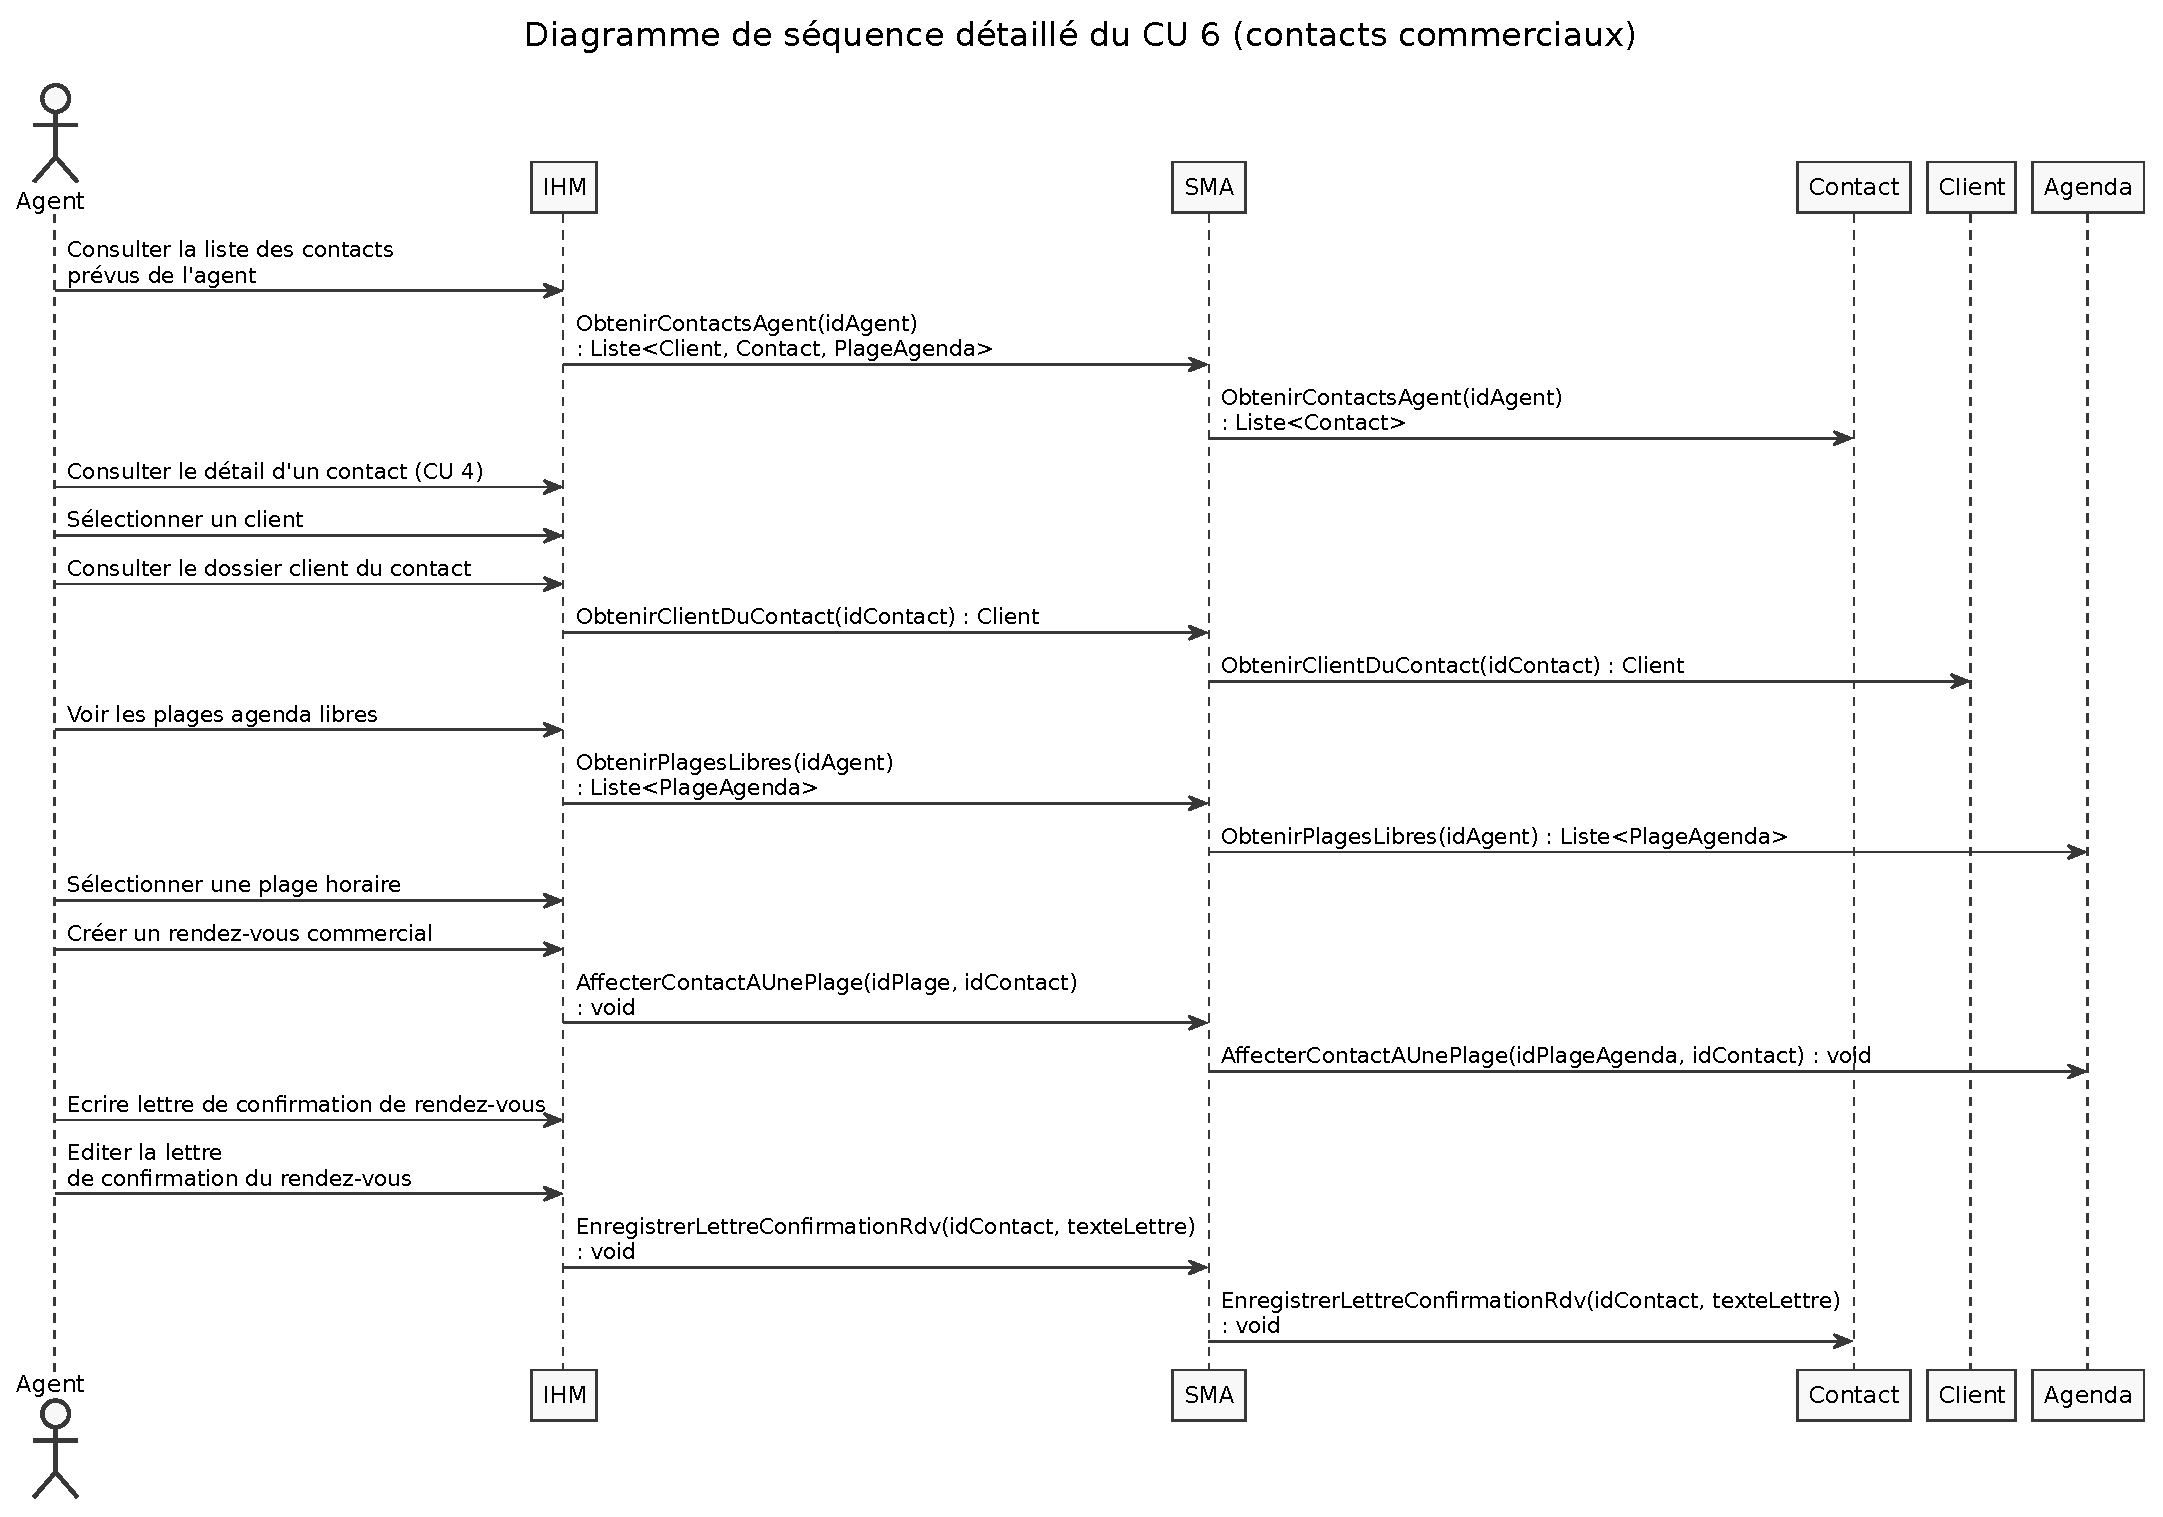
\includegraphics[width=23cm, angle=90]{figures/eps/DSD_CU6_partieAgent.eps}}
\caption{DSD "contacts commerciaux" du CU6}
\end{figure}

\subsection{Partie Client}
\begin{figure}[H]
\centering
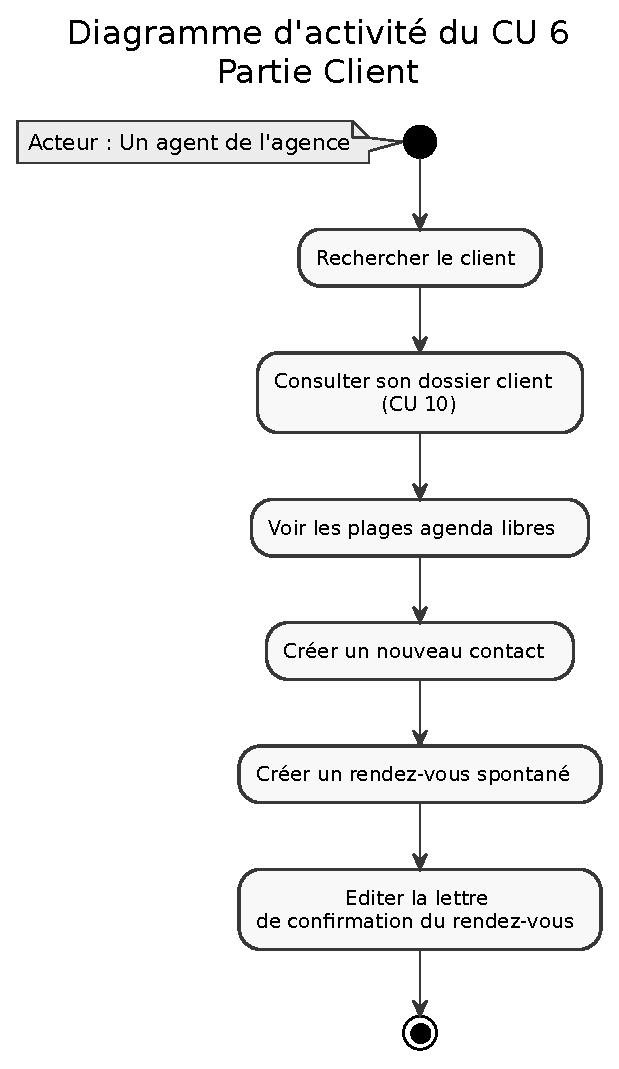
\includegraphics[width=10cm]{figures/eps/DA_CU6_partieClient.eps}
\caption{DA du CU6}
\end{figure}

\begin{figure}[H]
\noindent\makebox[\textwidth]{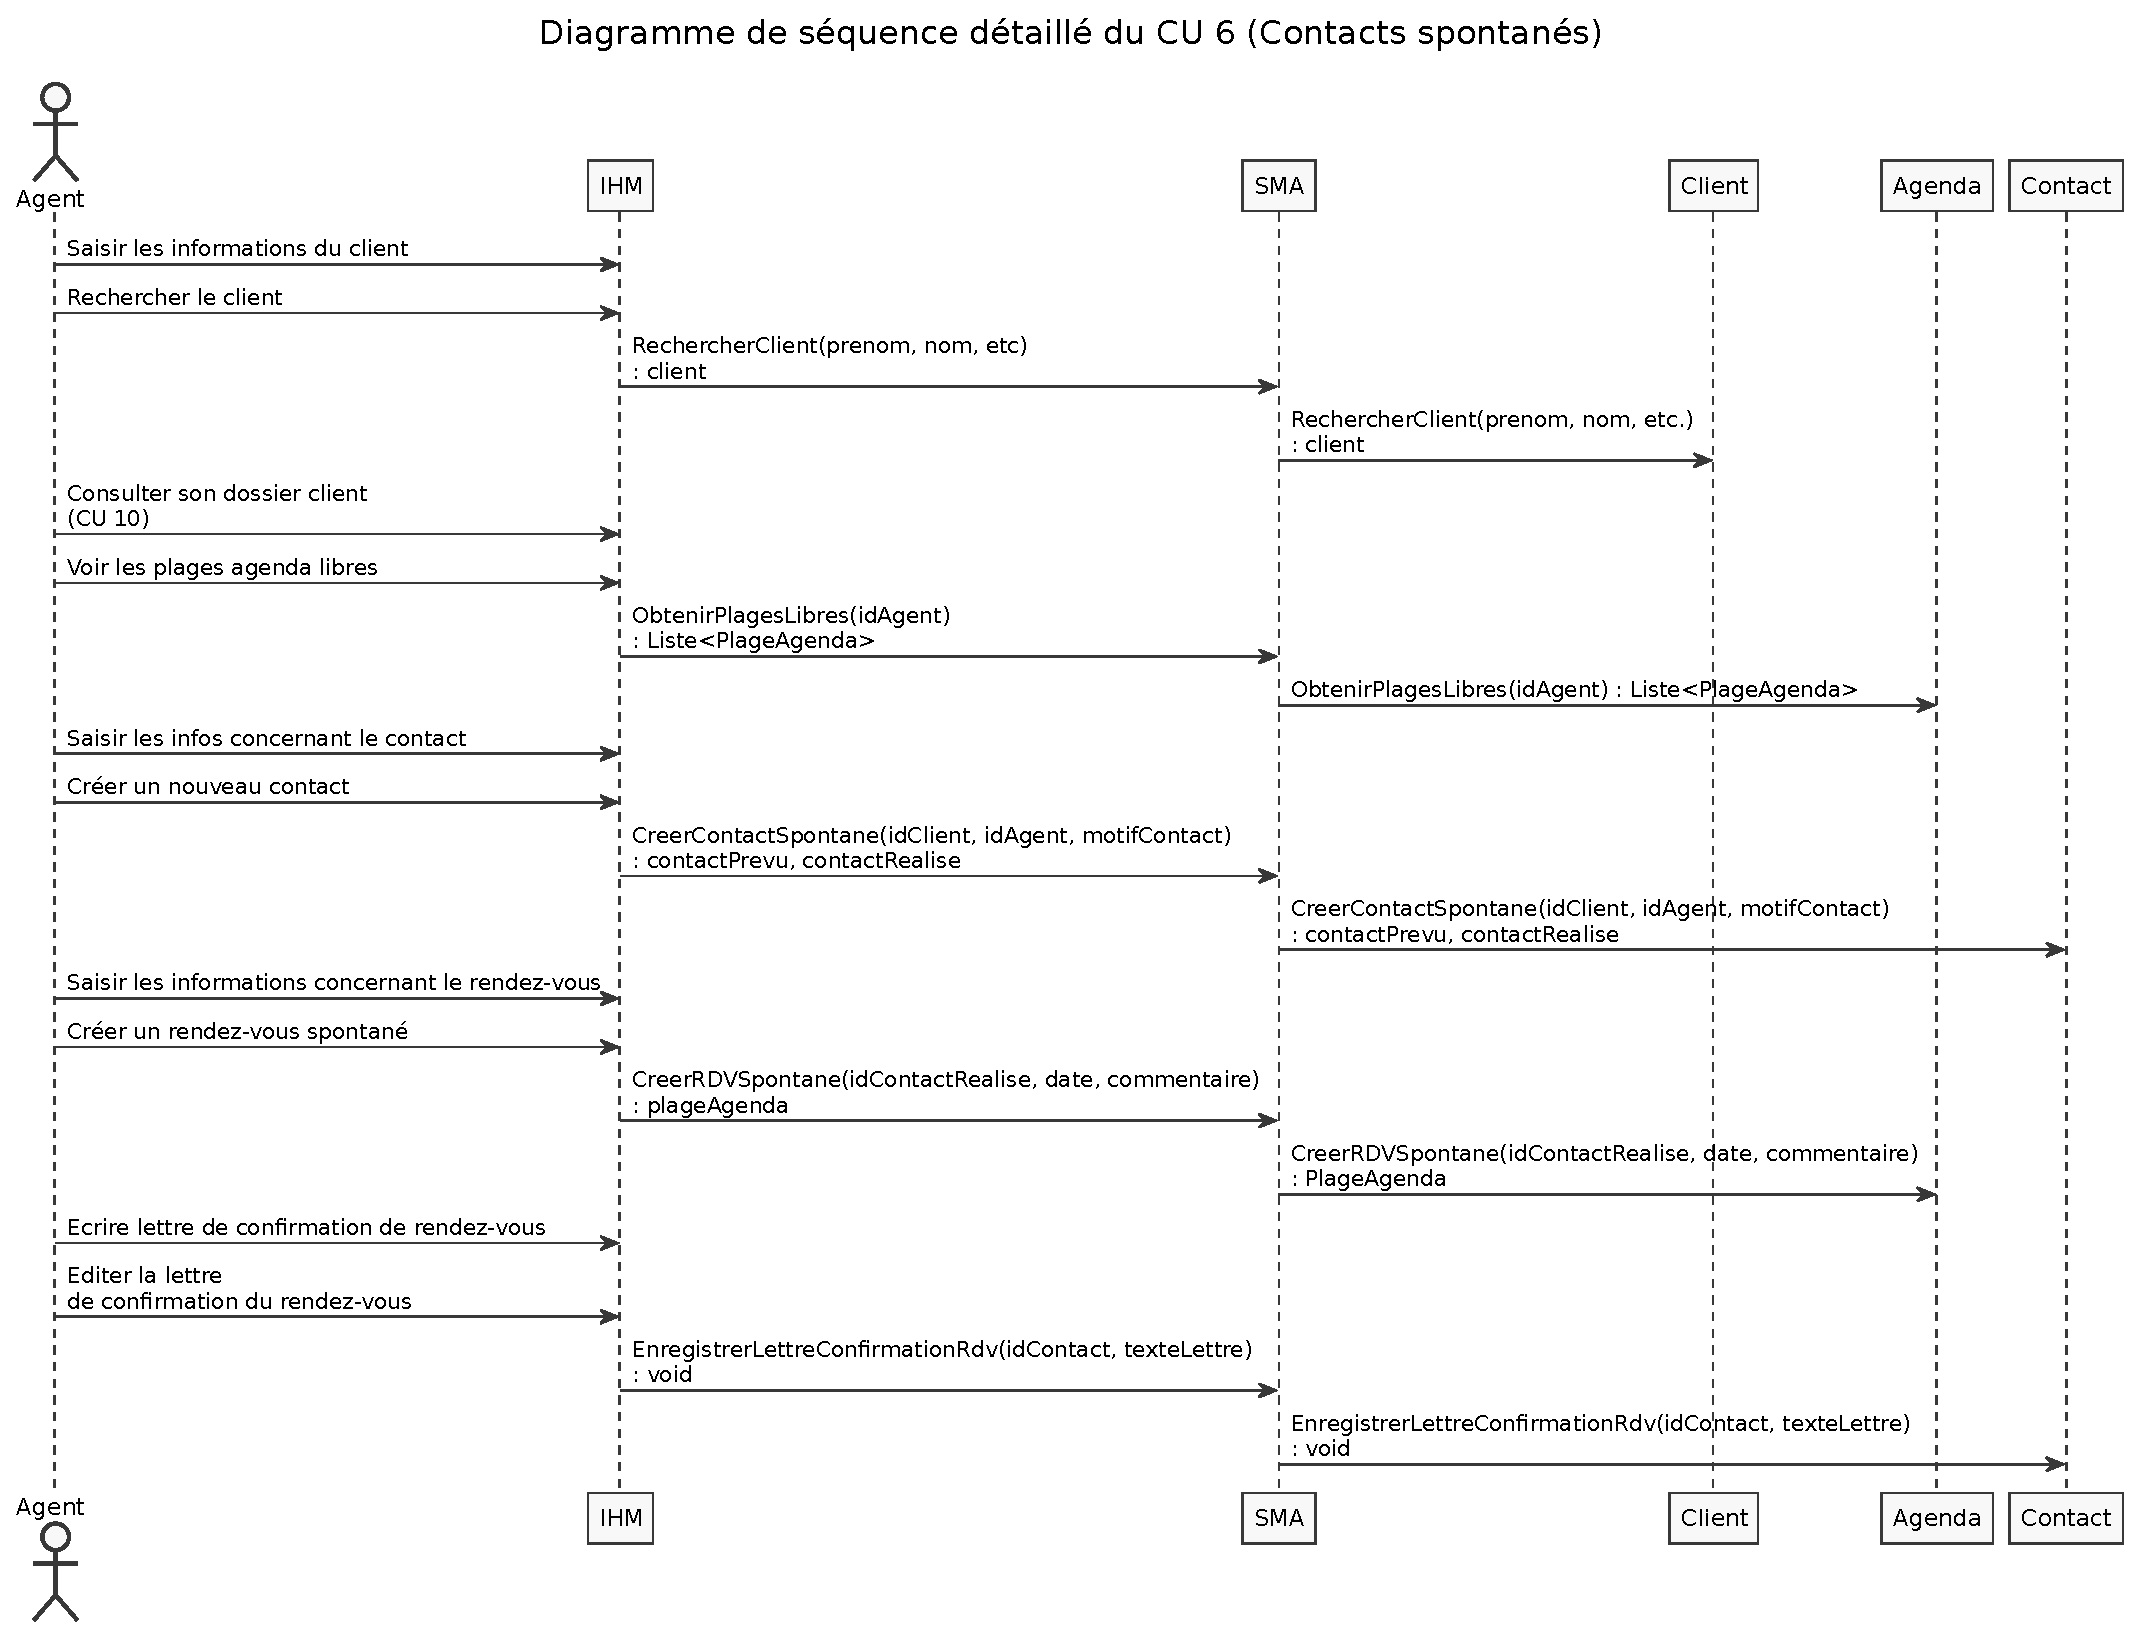
\includegraphics[width=23cm, angle=90]{figures/eps/DSD_CU6_partieClient.eps}}
\caption{DSD "contacts spontanés" du CU6}
\end{figure}

\clearpage
\section{CU7 - Consultation des agendas}
\begin{figure}[H]
\centering
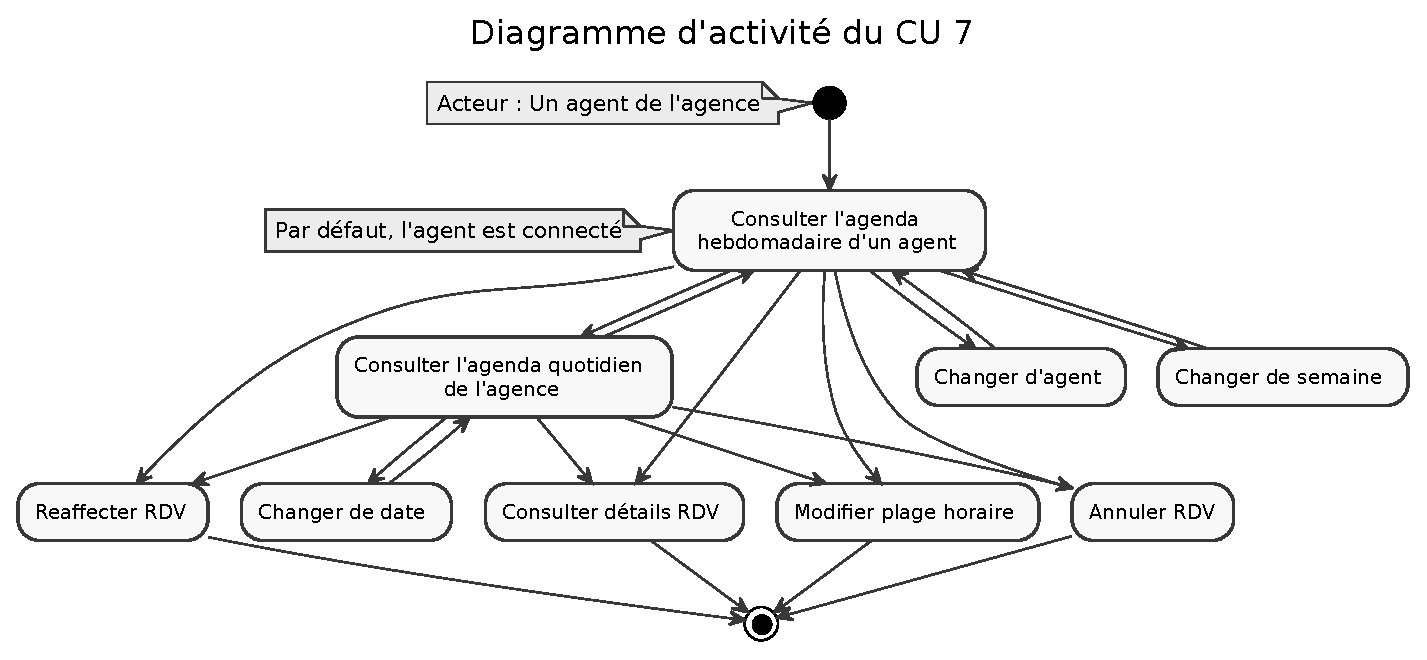
\includegraphics[width=20cm, angle=90]{figures/eps/DA_CU7.eps}
\caption{DA du CU7}
\end{figure}


\begin{figure}[H]
\noindent\makebox[\textwidth]{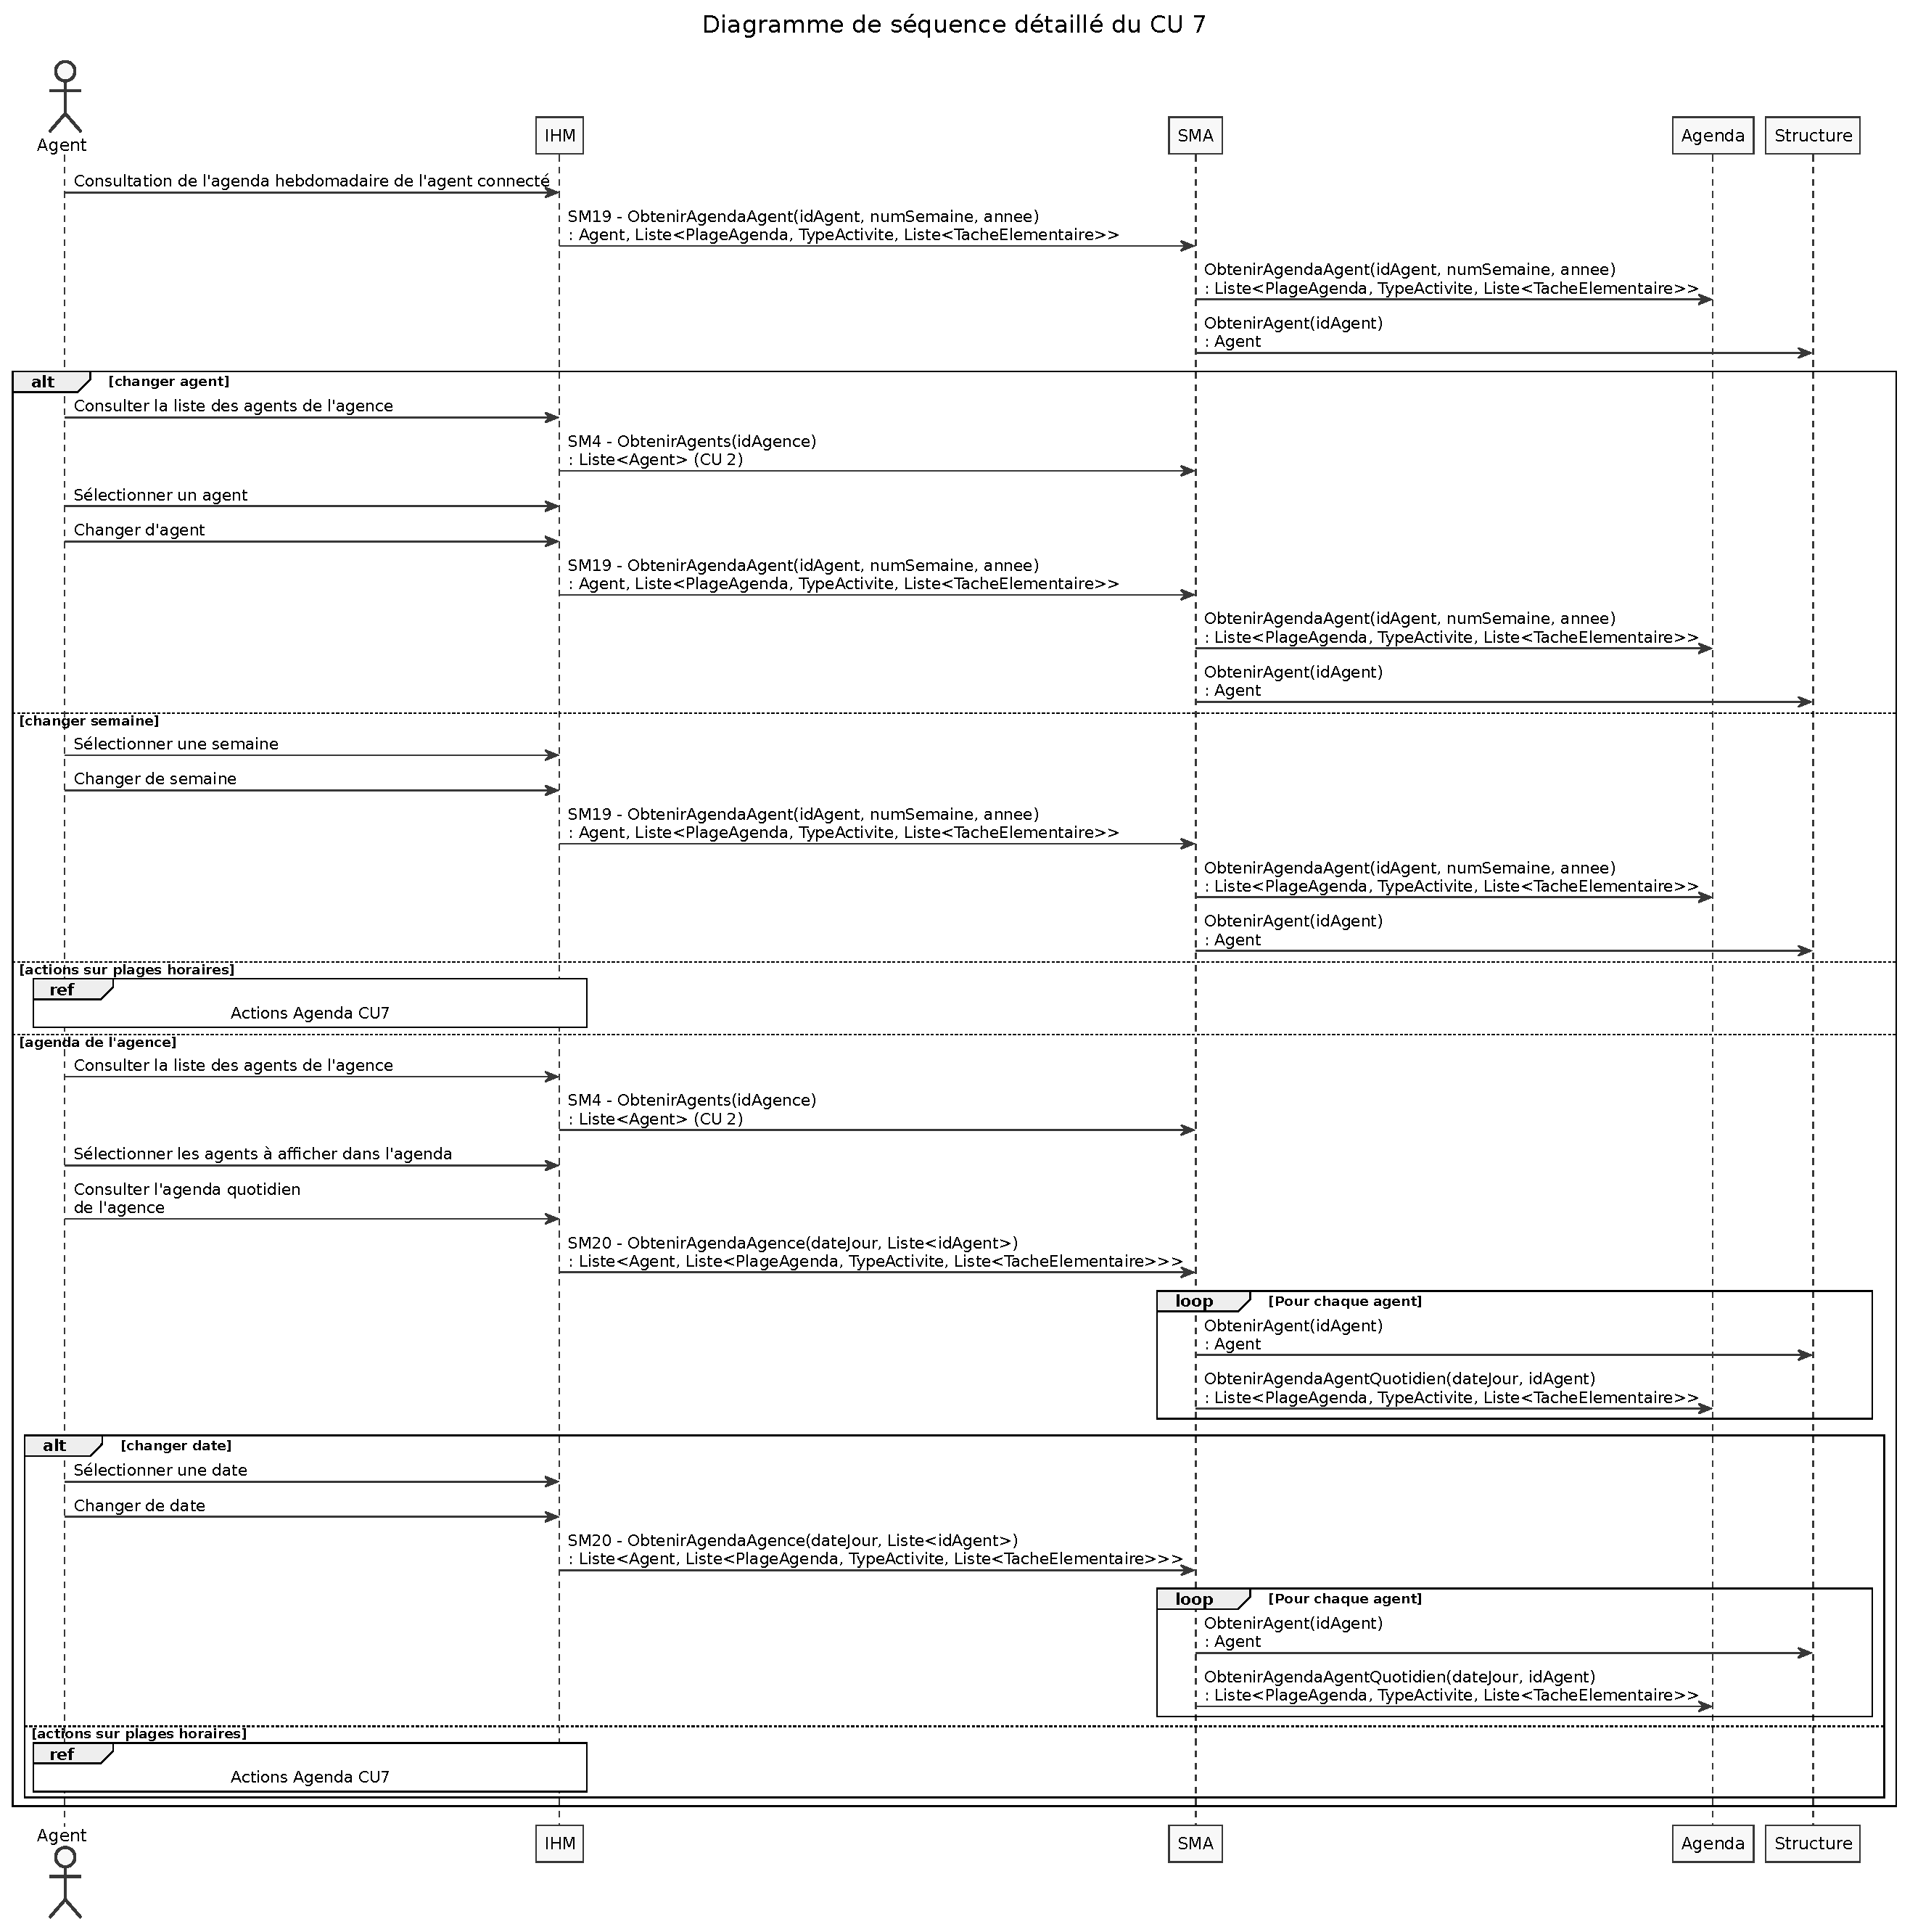
\includegraphics[width=19cm]{figures/eps/DSD_CU7.eps}}
\caption{DSD du CU7}
\end{figure}

\begin{figure}[H]
\noindent\makebox[\textwidth]{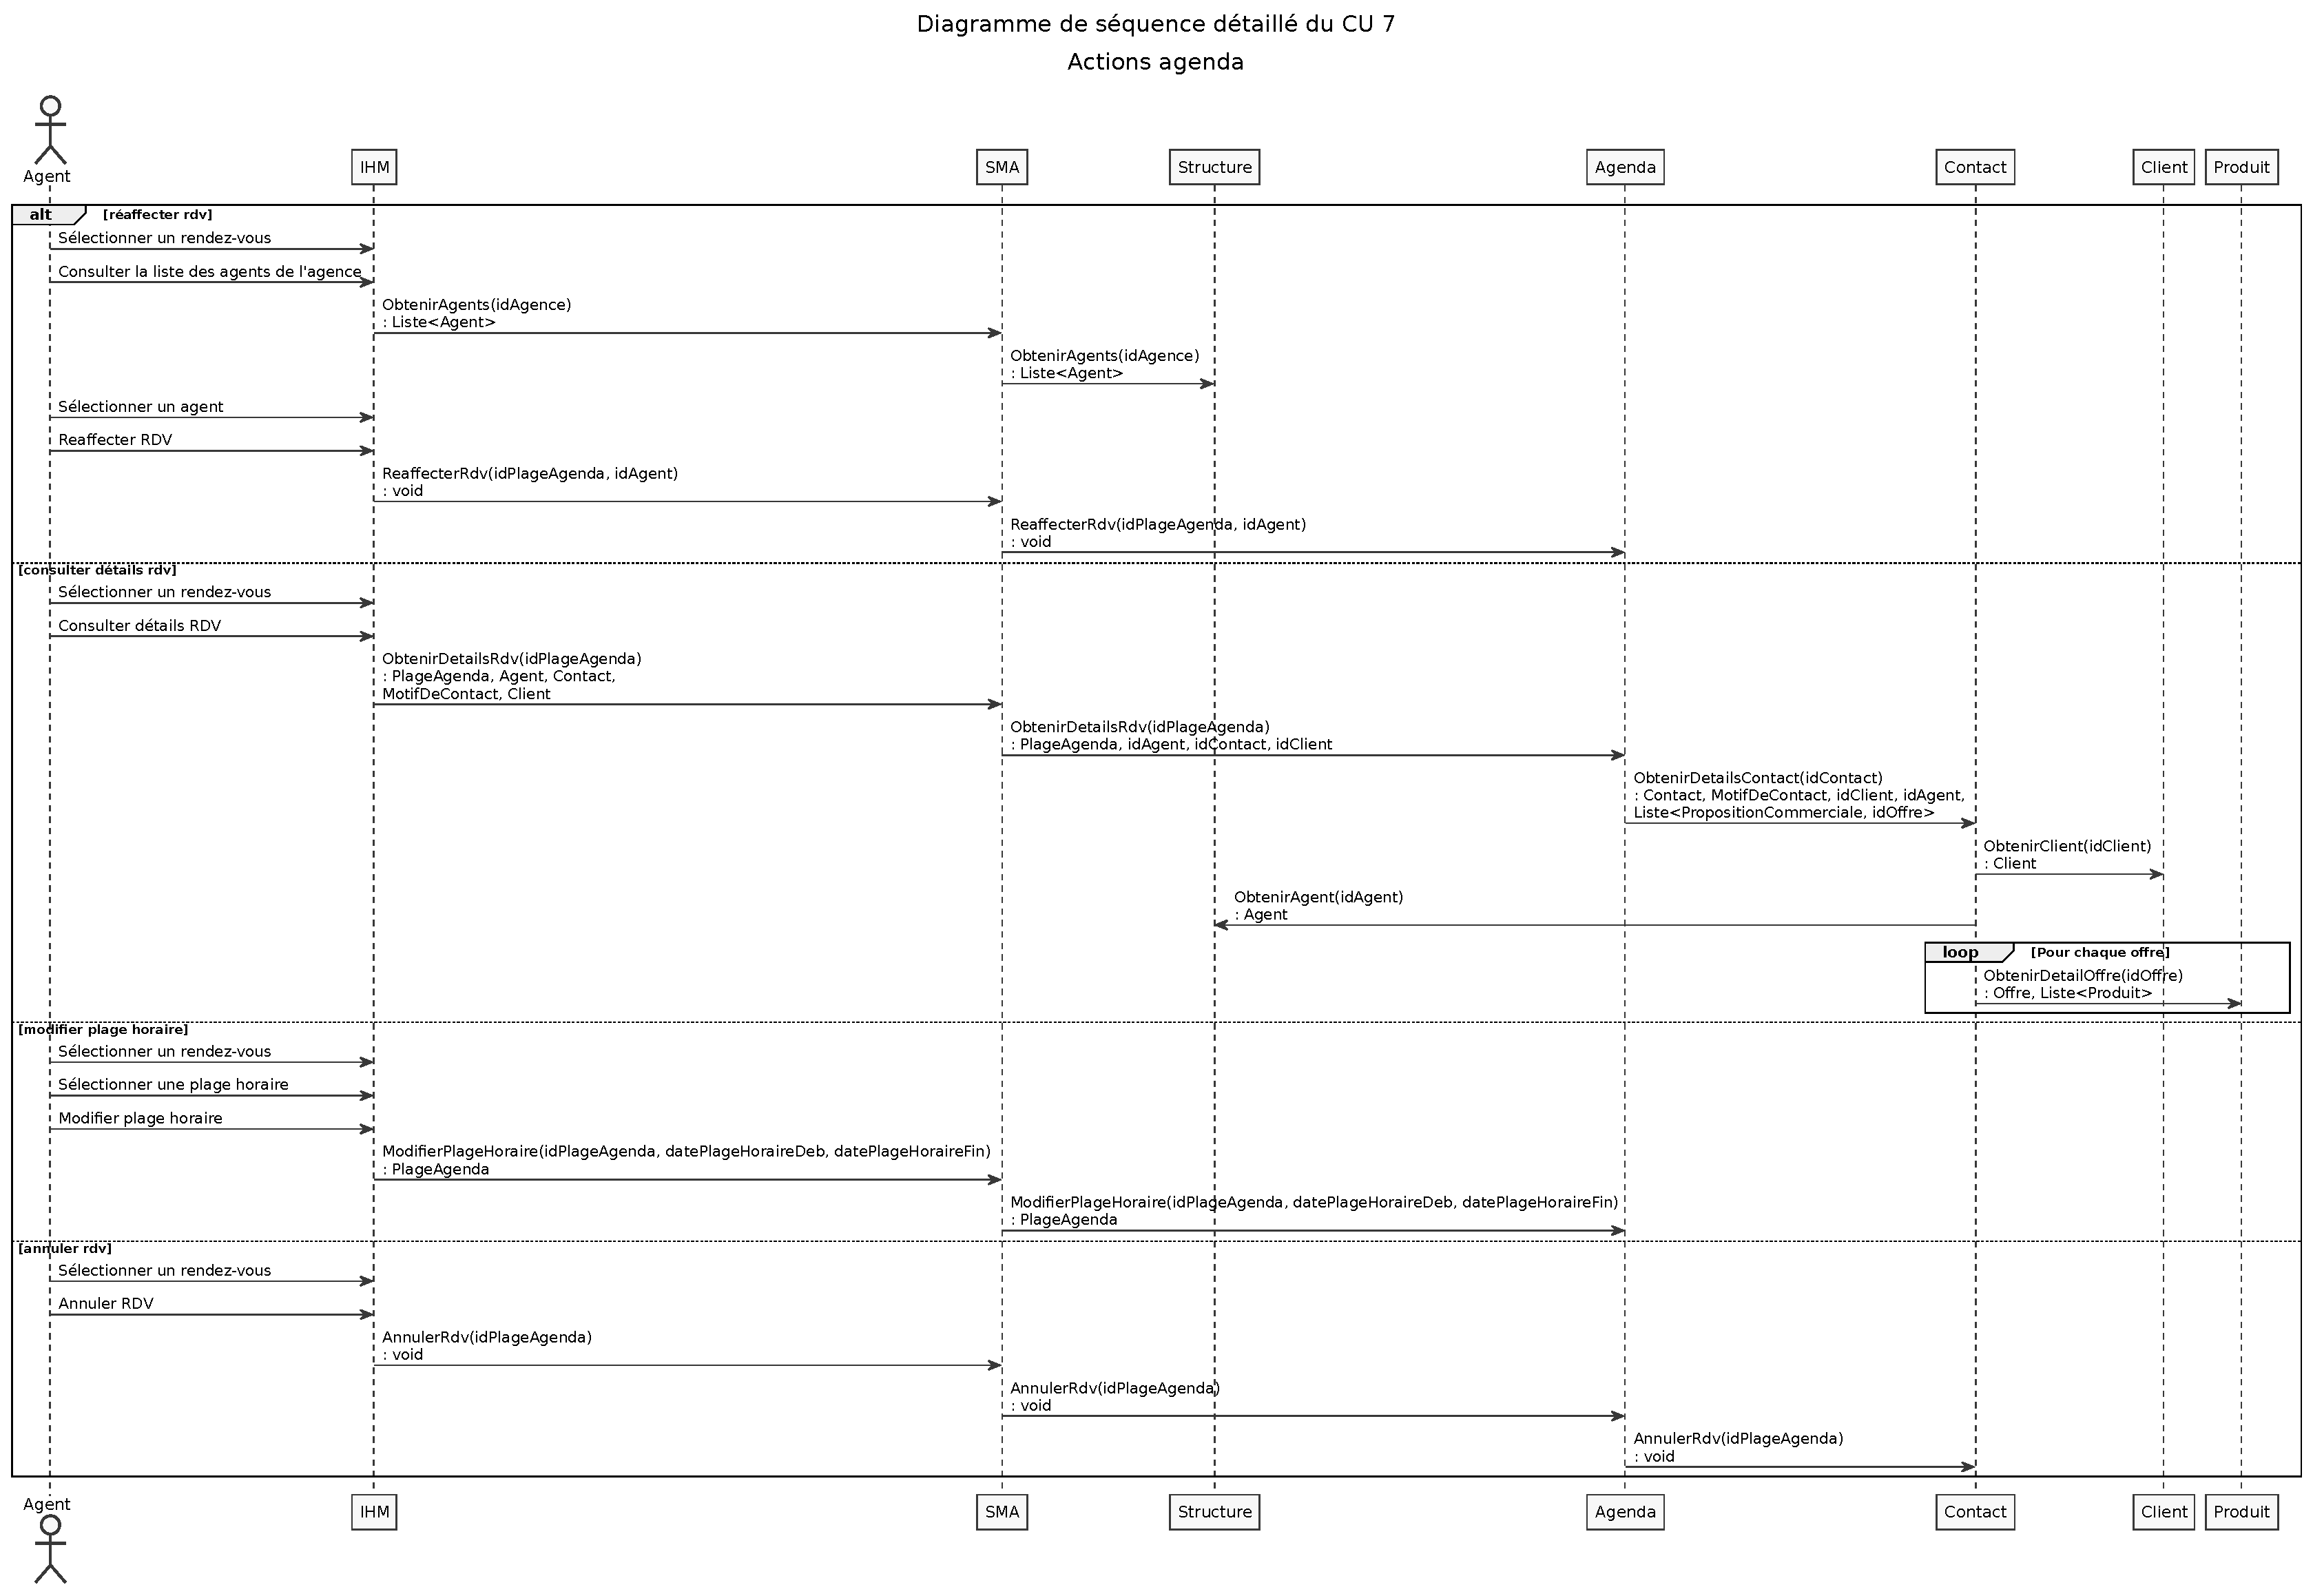
\includegraphics[width=24cm, angle=90]{figures/eps/DSD_CU7_ActionsAgenda}}
\caption{DSD "Actions Agenda" du CU7}
\end{figure}

\clearpage
\section{CU8 - Préparation d’entretien par un agent}

\begin{figure}[H]
\centering
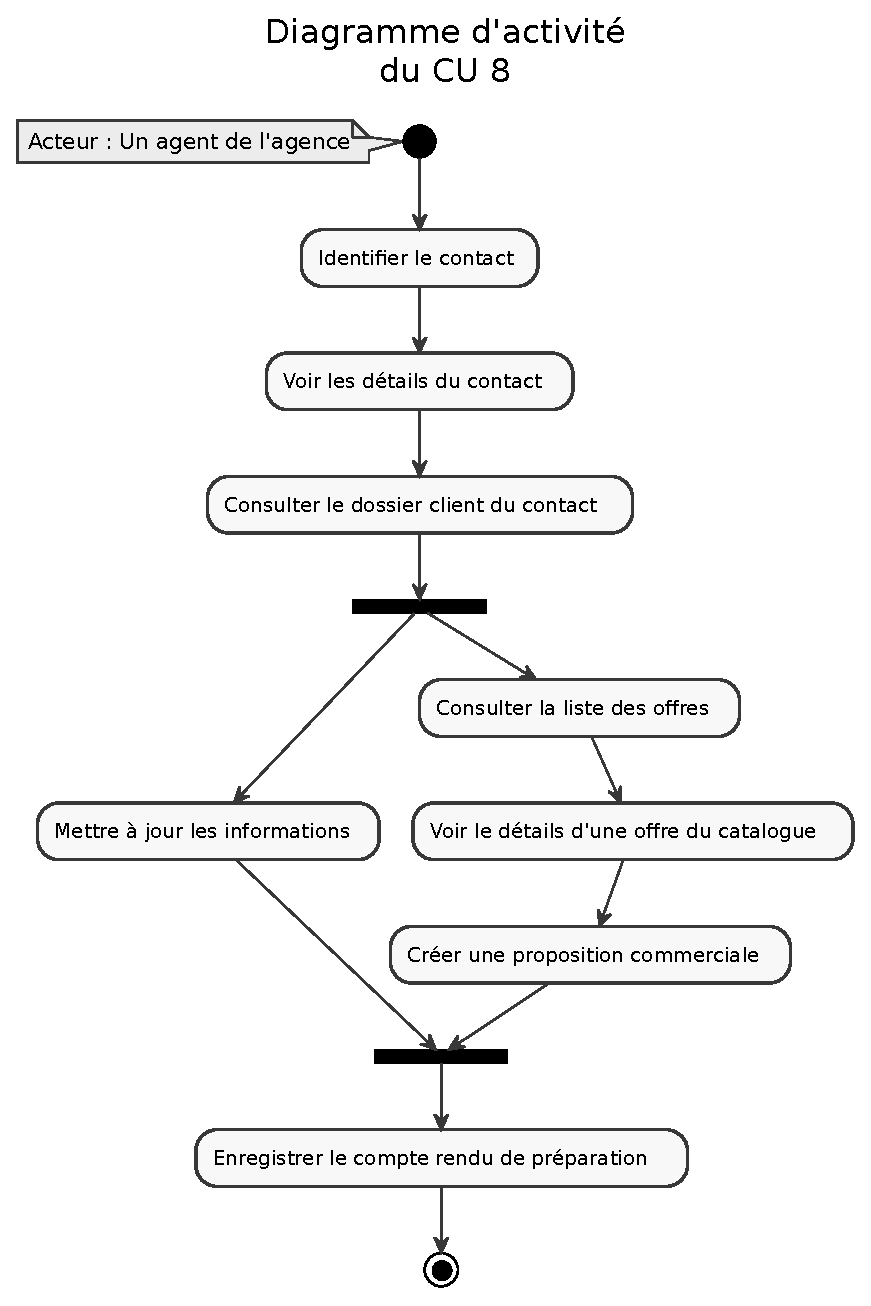
\includegraphics[width=10cm]{figures/eps/DA_CU8.eps}
\caption{DA du CU8}
\end{figure}

\begin{figure}[H]
\noindent\makebox[\textwidth]{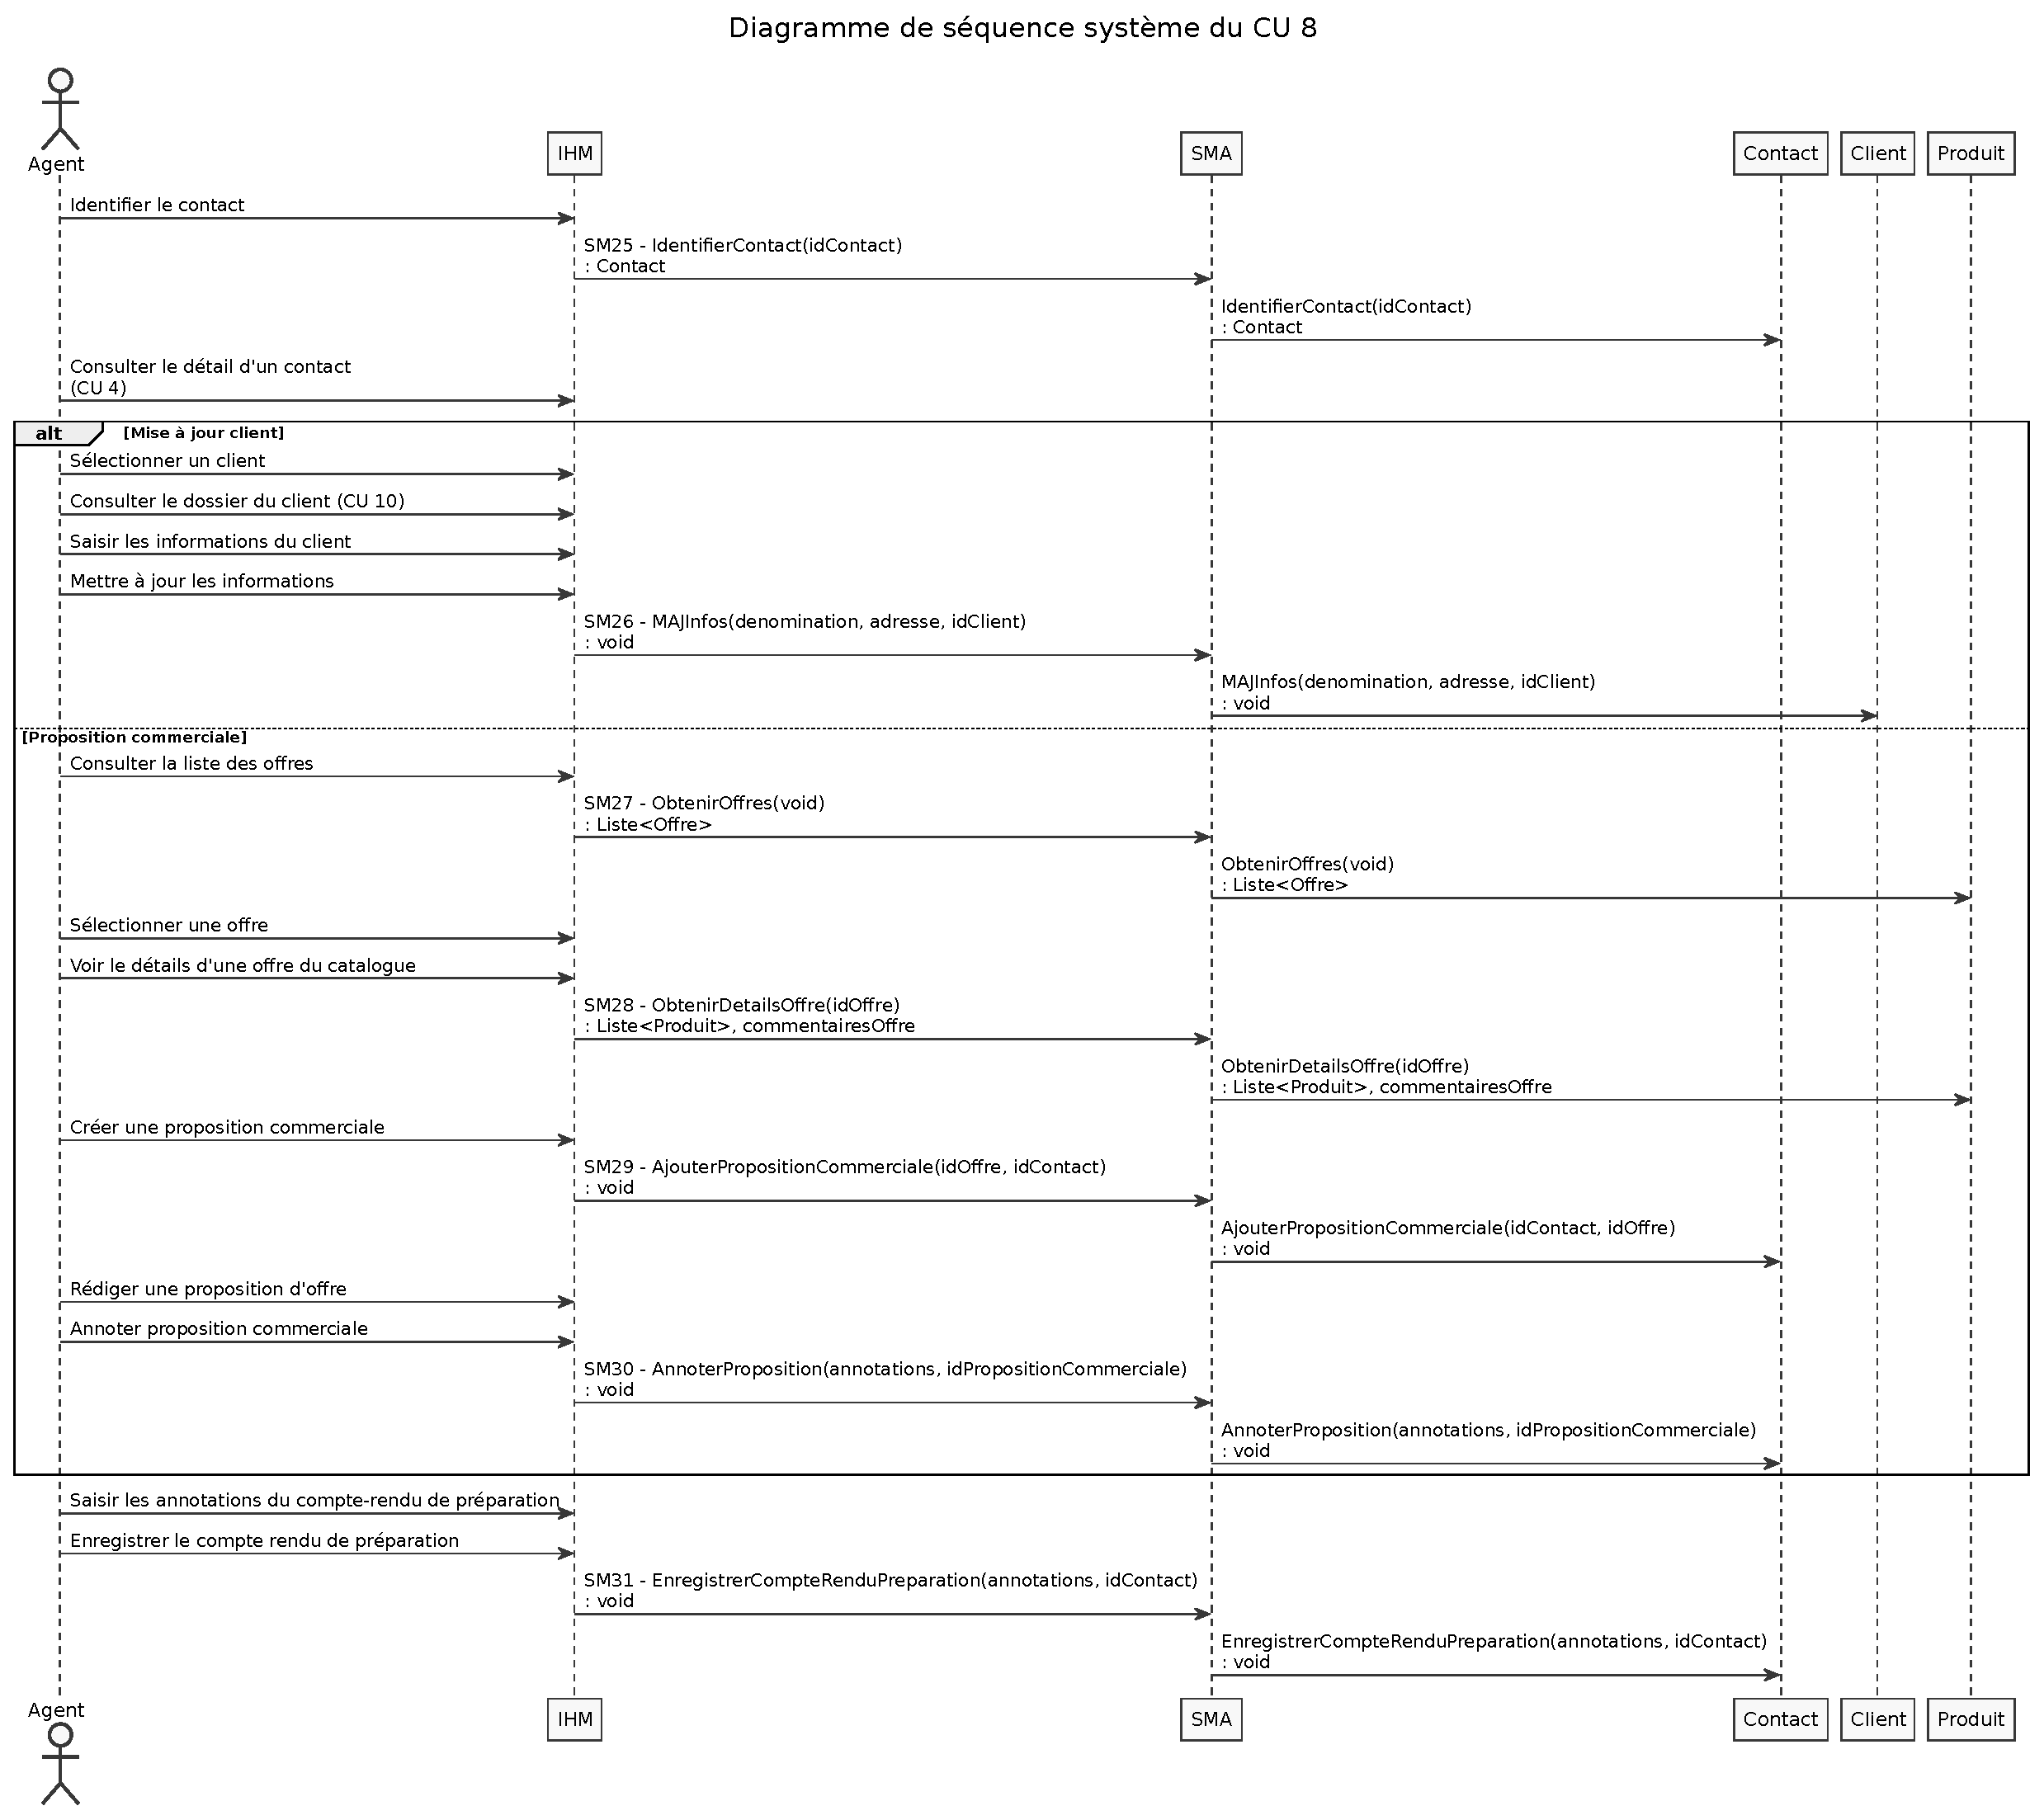
\includegraphics[width=22cm, angle=90]{figures/eps/DSD_CU8.eps}}
\caption{DSD du CU8}
\end{figure}

\clearpage
\section{CU9 - Conduite de l’entretien par l’agent}

\begin{figure}[H]
\centering
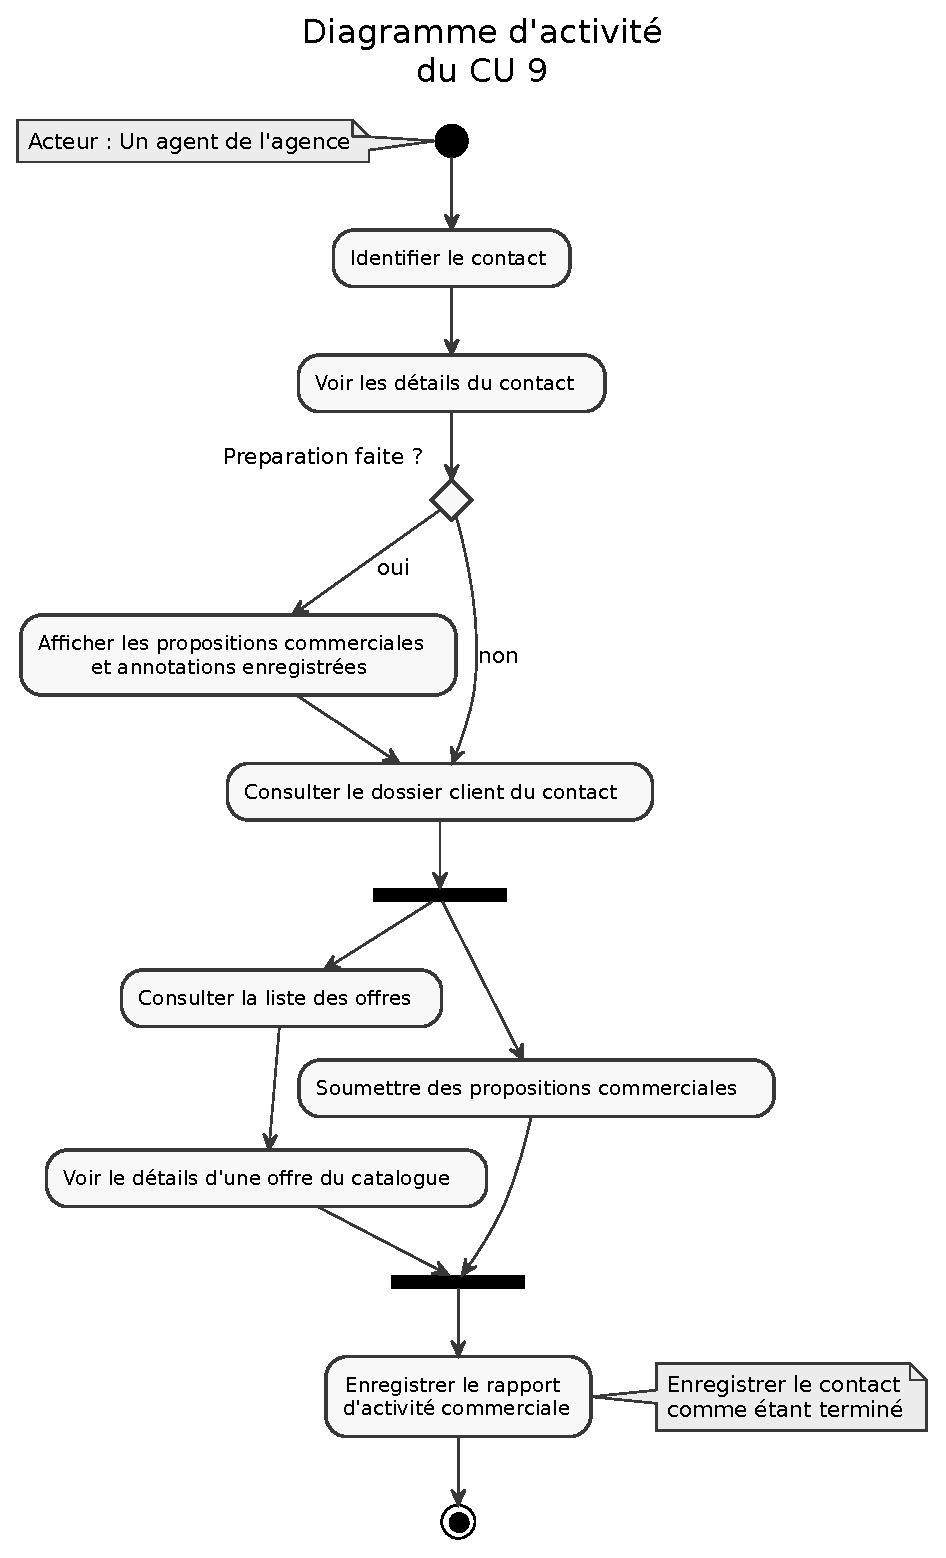
\includegraphics[width=10cm]{figures/eps/DA_CU9.eps}
\caption{DA du CU9}
\end{figure}

\begin{figure}[H]
\noindent\makebox[\textwidth]{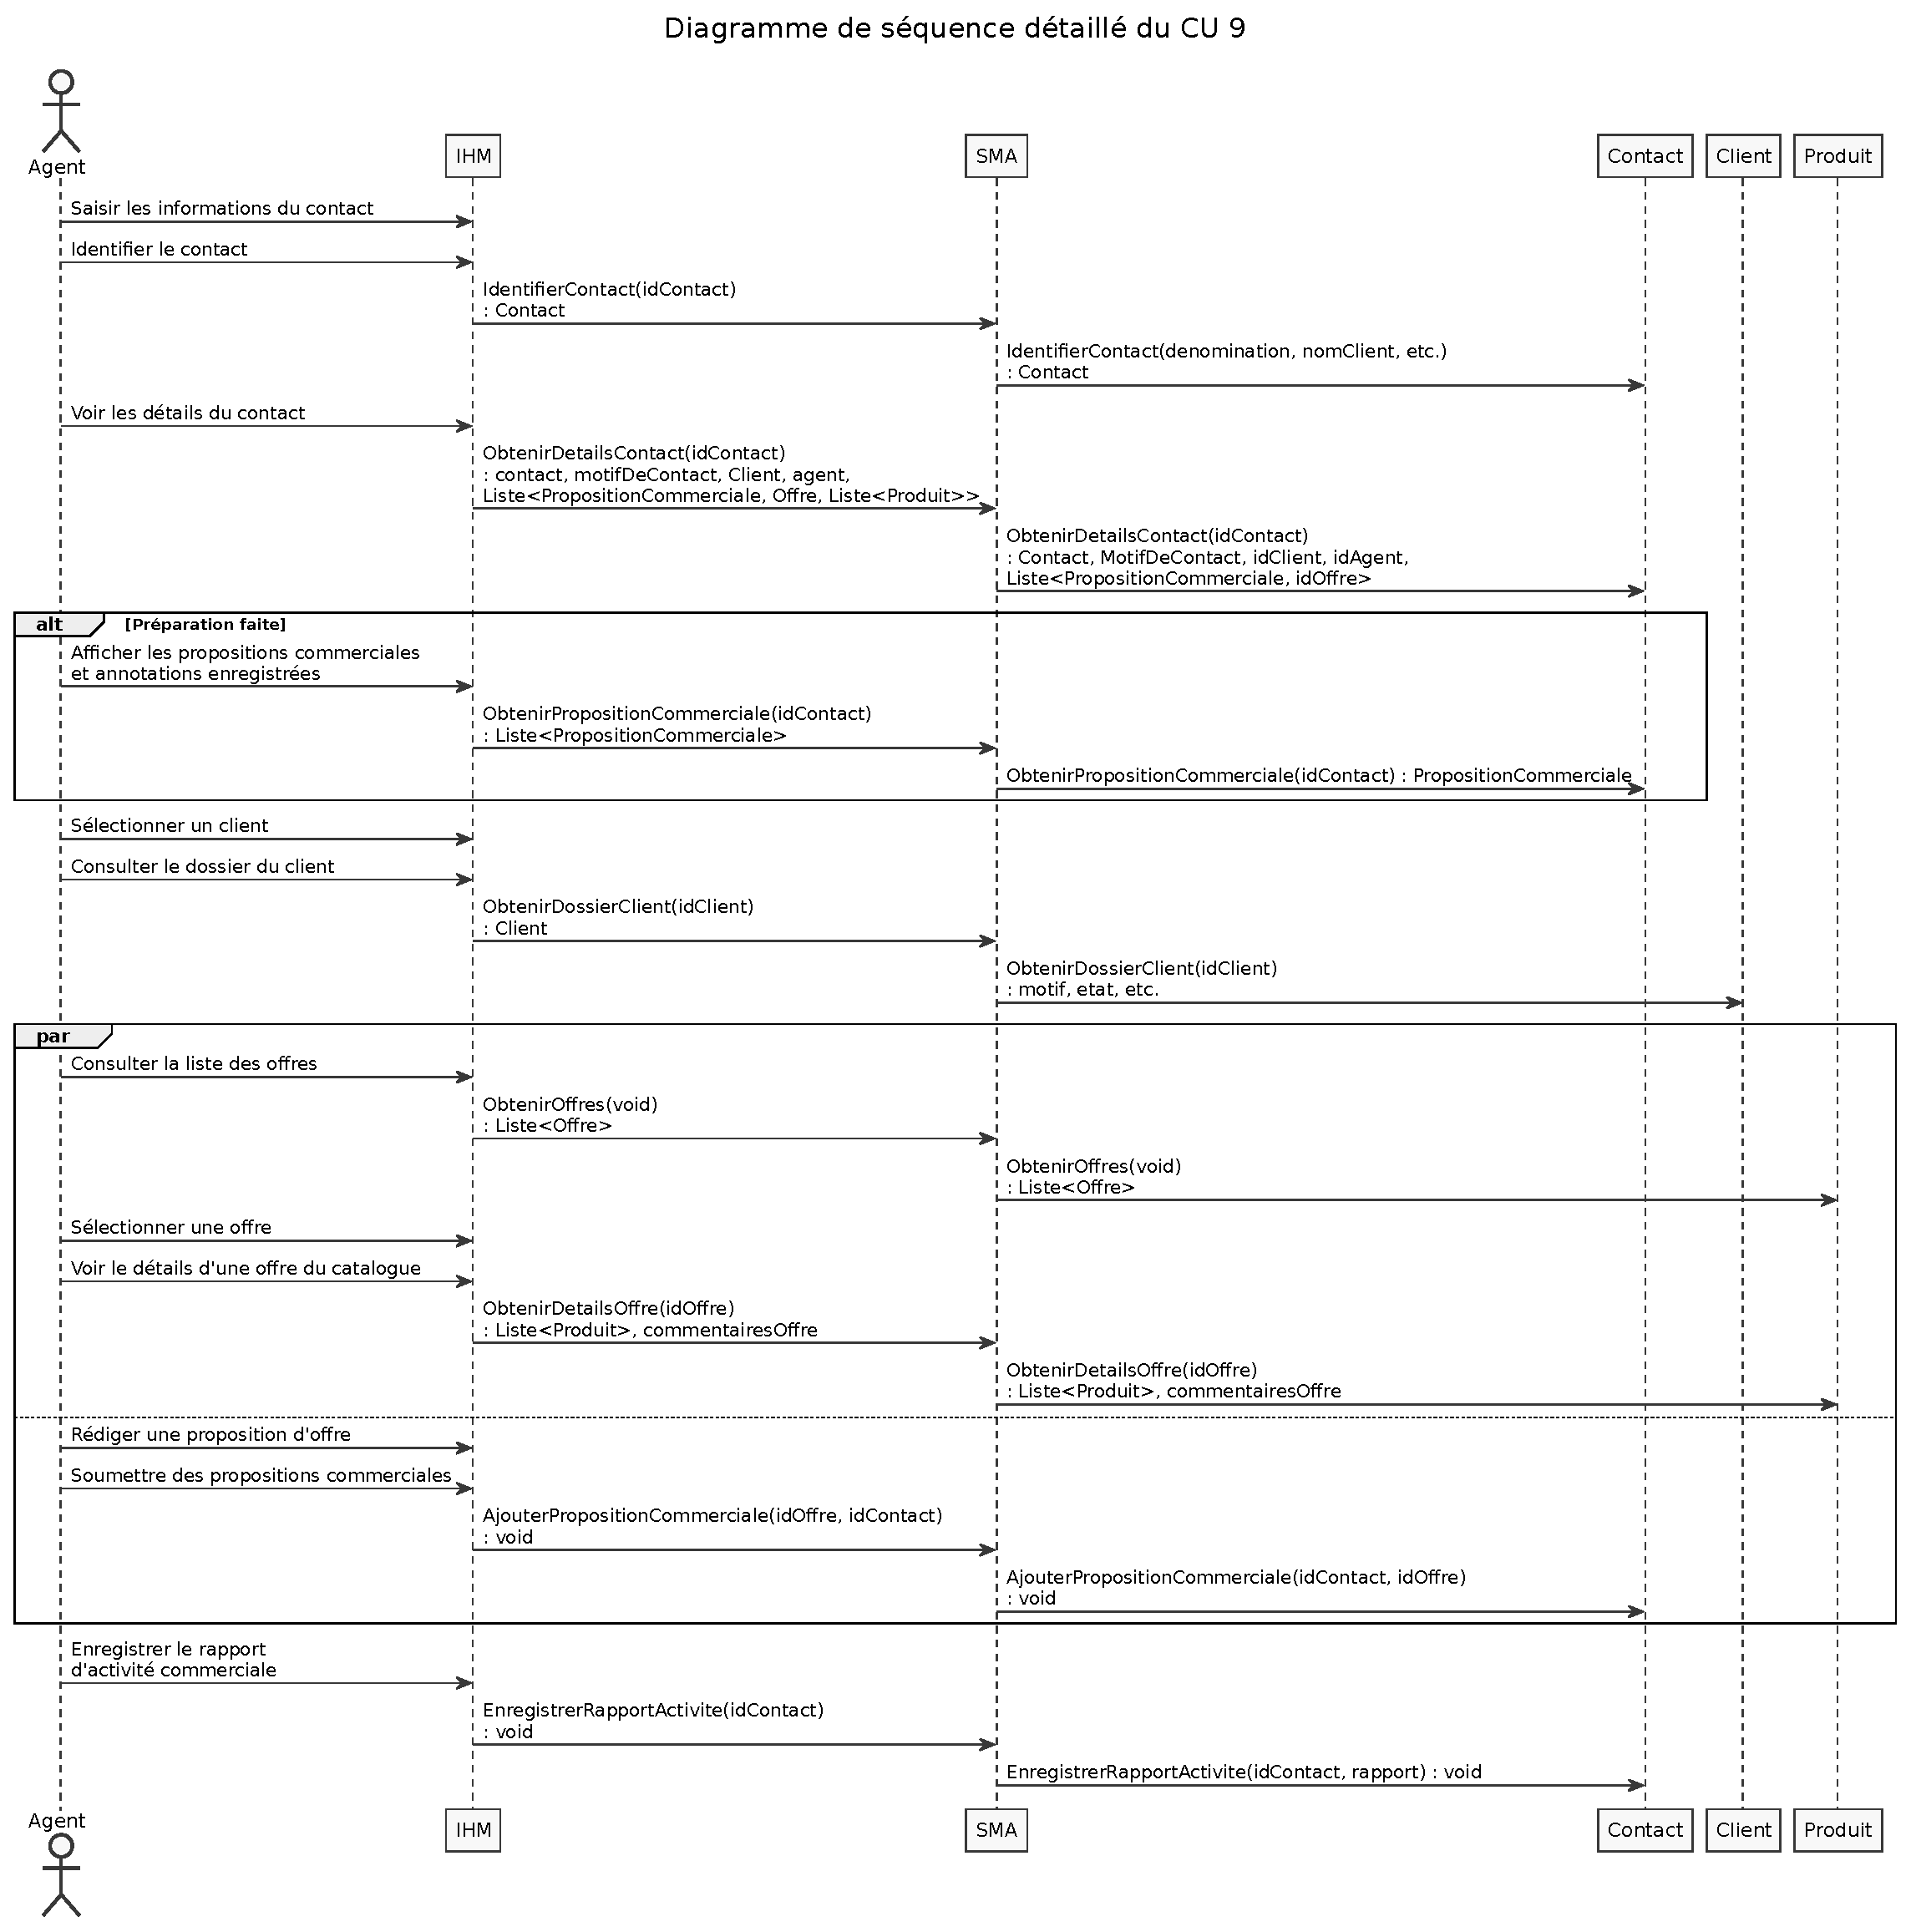
\includegraphics[width=19.5cm, angle=90]{figures/eps/DSD_CU9.eps}}
\caption{DSD du CU9}
\end{figure}

\clearpage
\section{CU10 - Consultation du dossier client}
\begin{figure}[H]
\centering
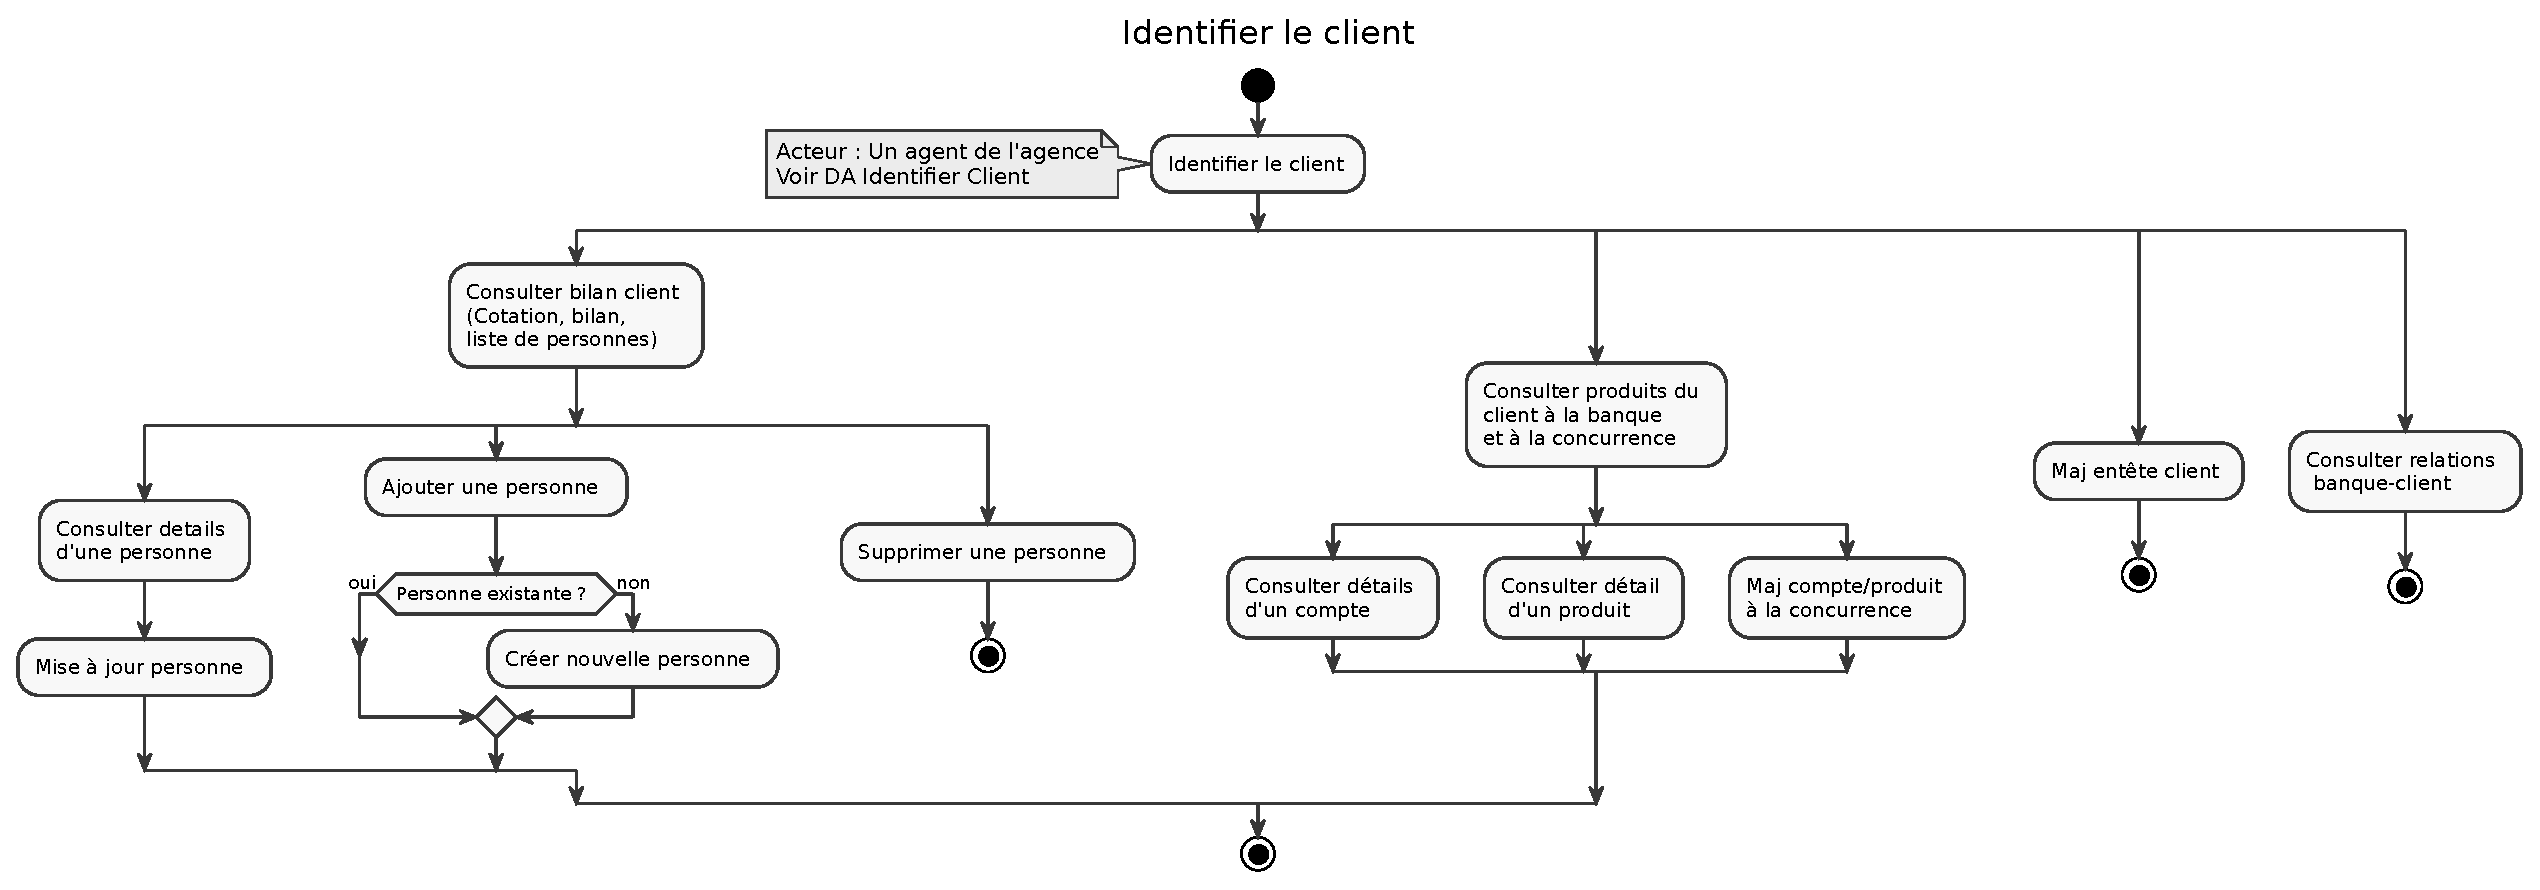
\includegraphics[width=22cm, angle=90]{figures/eps/DA_CU10.eps}
\caption{DA du CU10}
\end{figure}


\begin{figure}[H]
\noindent\makebox[\textwidth]{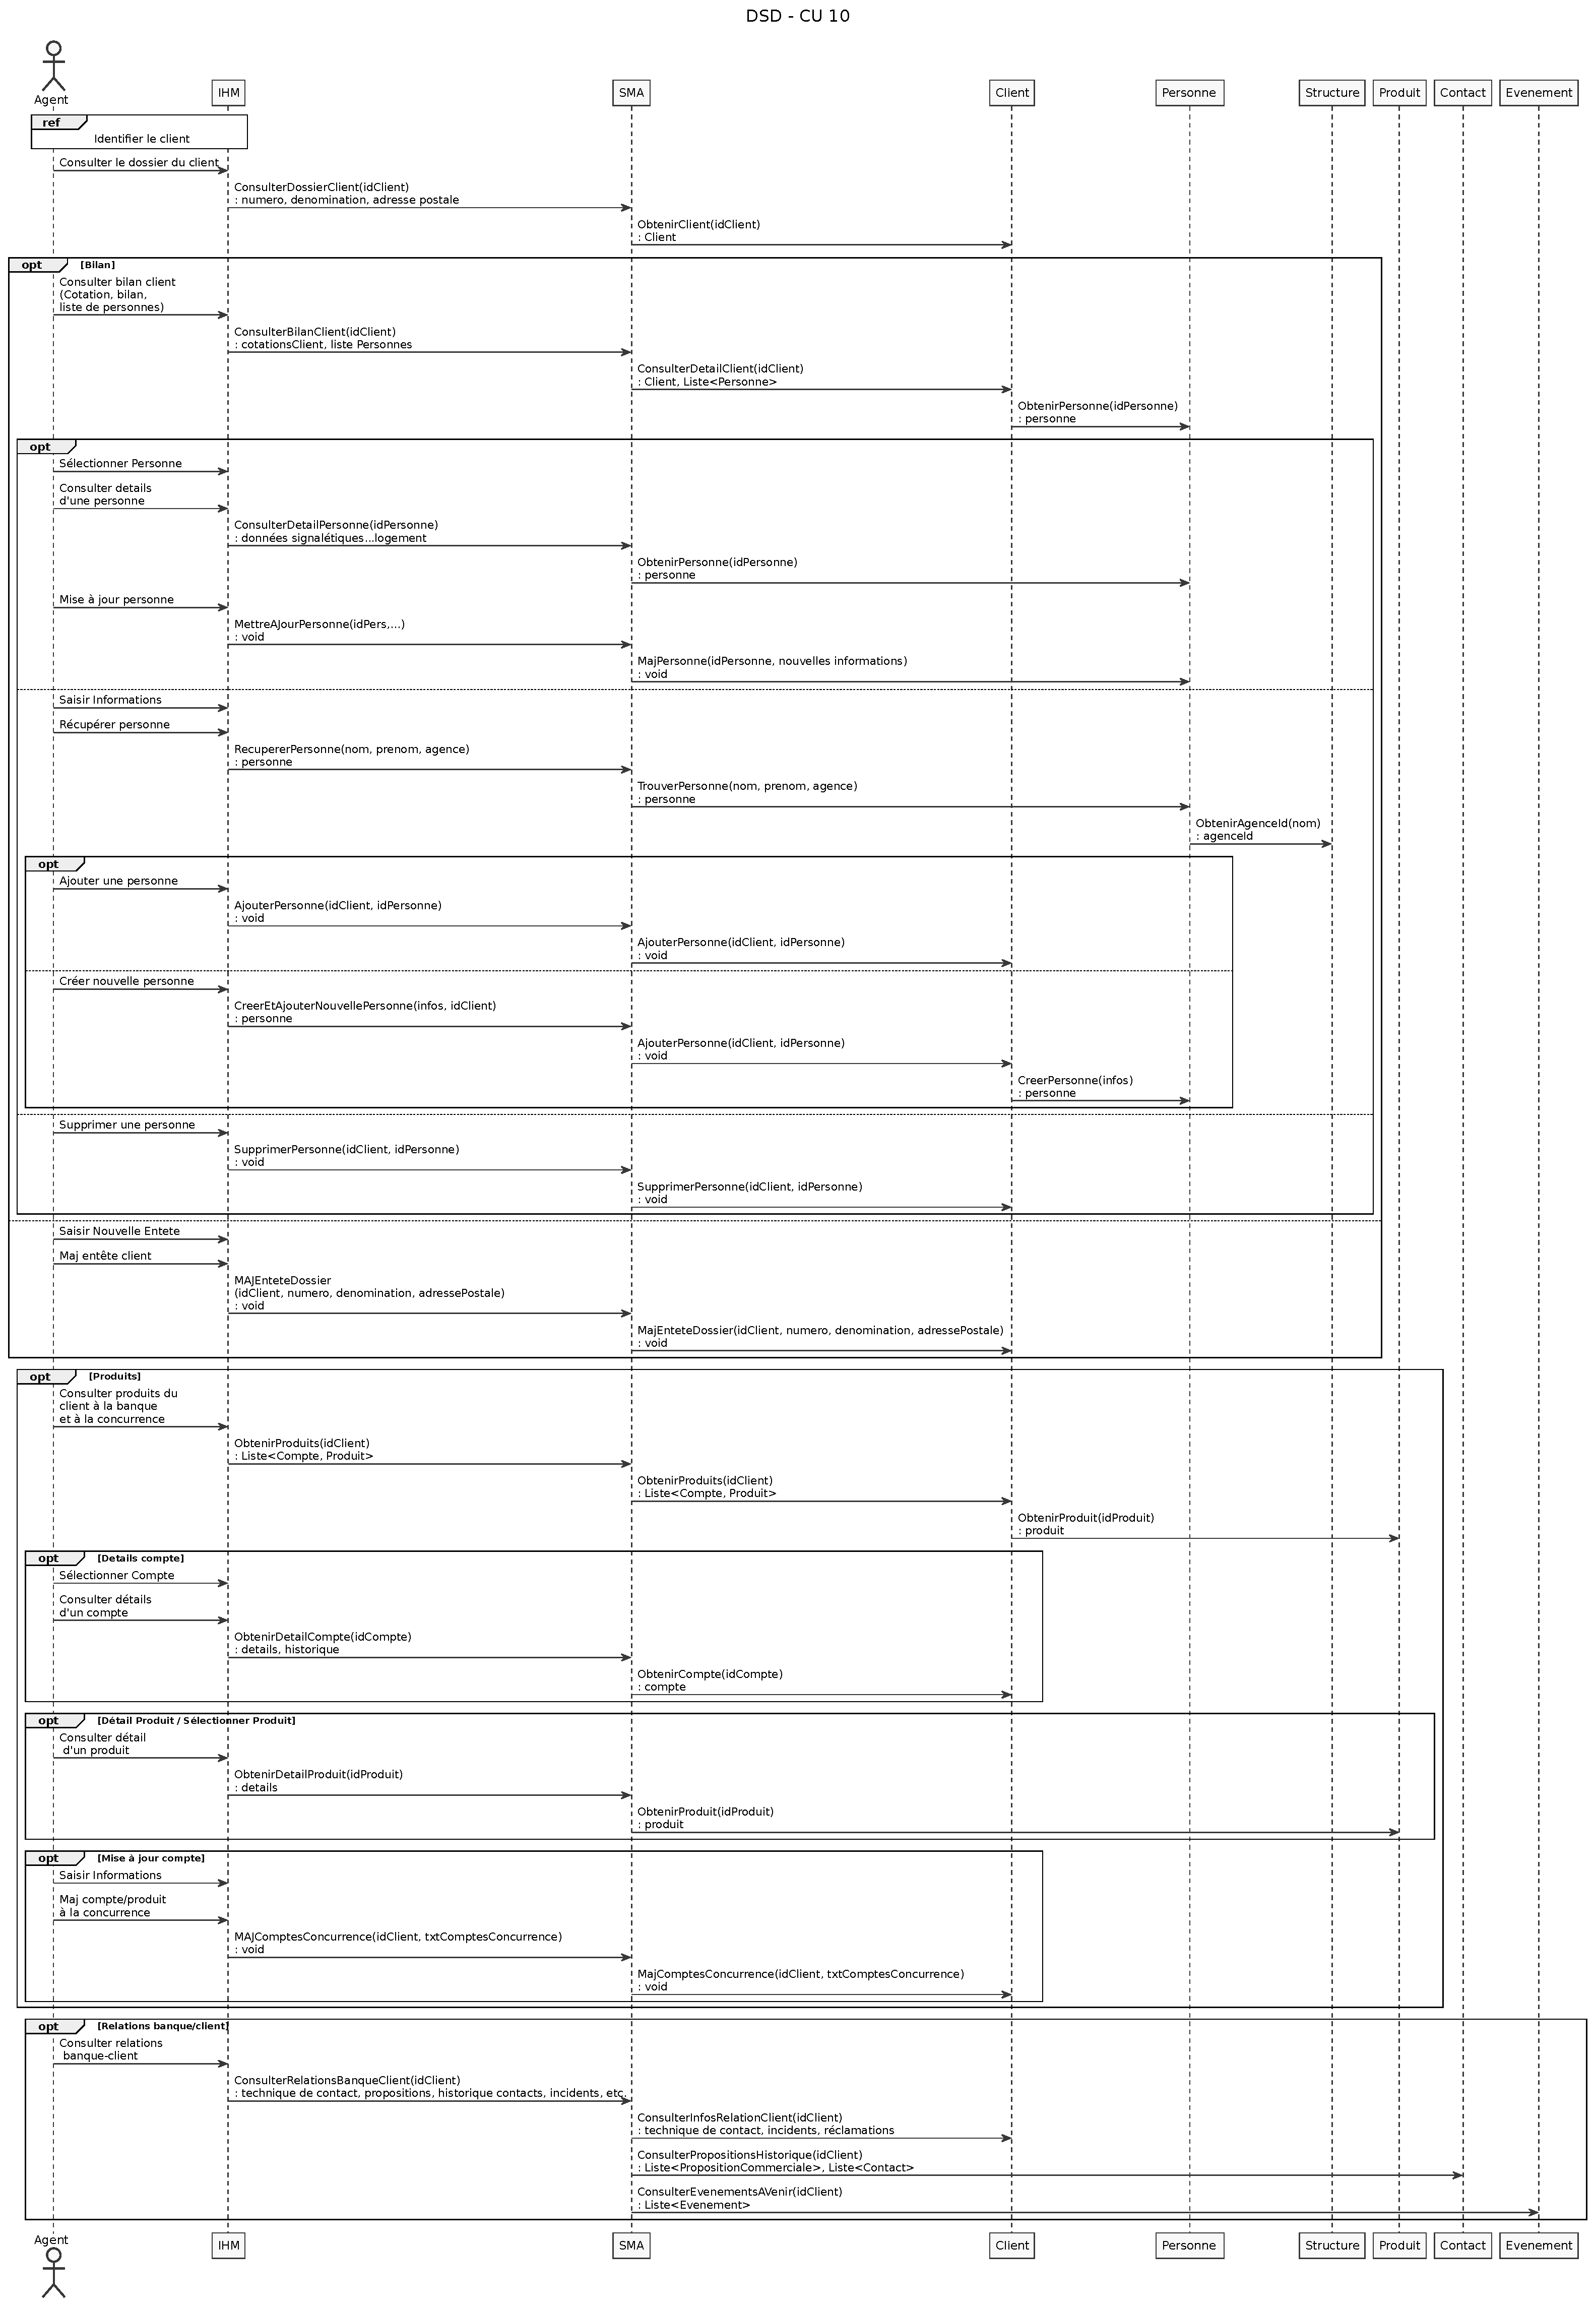
\includegraphics[width=18cm]{figures/eps/DSD_CU10.eps}}
\caption{DSD du CU10}
\end{figure}
